%%{ DOC HEAD

% \newcommand*{\printversion}{}%
% \newcommand*{\includepdfs}{}%

\pdfoutput=1
\ifdefined\printversion
  \documentclass[a4paper,11pt,twoside,openright]{book}
\else
  \documentclass[a4paper,11pt,oneside]{book}
\fi

\newcommand{\conditionalClearPage}{
  \ifdefined\printversion
    \cleardoublepage
  \else
    \clearpage
  \fi
}

\usepackage[english]{babel}
\usepackage[utf8]{inputenc}
\usepackage{csquotes}

\usepackage{amsmath,amsfonts,amssymb,bm}
\usepackage{nicefrac}

\usepackage{algorithm,algpseudocode}
\usepackage[title,titletoc]{appendix}
\usepackage{latexsym}
\usepackage{a4wide}
\usepackage{color}
\usepackage{indentfirst}
\usepackage{graphicx}       %%% graphics for dvips
\usepackage{fancyhdr,lastpage}
\usepackage{longtable}
\usepackage{pifont}
\usepackage{makeidx}
\usepackage{multirow}
\usepackage{dcolumn}
\usepackage{epstopdf}
\usepackage{url}
\usepackage{listings}
\usepackage{relsize}
\usepackage{pdfpages}
\usepackage{url}
\usepackage{lipsum}
\usepackage{isotope}
\usepackage{verbatim}
\usepackage{xcolor}
\usepackage{tcolorbox}
\usepackage[hidelinks]{hyperref}

\usepackage{subfig} % subfloat
\usepackage[export]{adjustbox}

\hyphenation{}

%%{ tikz

\usepackage{tikz}
\usepackage{pgfplots}
\pgfplotsset{compat=1.14}
\usetikzlibrary{backgrounds,arrows,automata,shapes,positioning,calc,through,spy,shapes,shapes.geometric,shapes.multipart,fit,patterns,fadings}
\pgfdeclarelayer{background}
\pgfdeclarelayer{foreground}
\pgfsetlayers{background,main,foreground}

\tikzset{
    imgletter/.style={
      rectangle,
      inner sep=2pt,
      rounded corners=.1em,
      text=black,
      minimum height=1em,
      text centered,
      fill=white,
      fill opacity=1.0,
      text opacity=1,
      anchor=south west,
  },
}

%%}

%%{ include paper box

\newcommand{\includepaperwithimage}[1]{
  \ifdefined\includepdfs
    \includepdf[scale=0.85,pages=-,pagecommand={\thispagestyle{fancy}},offset=0.5cm 0cm]{./papers_to_include_pdf/#1}
  \else
    \clearpage
    \fullciteinboxwithimage{#1}{This place will contain the full paper}
  \fi
}

%%}

%%{ fullcite box

\definecolor{light-gray}{gray}{0.95}
\newcommand{\fullciteinbox}[2]{%

\DeclareCiteCommand{\fullcite}
{\usebibmacro{prenote}}
{\clearfield{addendum}%
  \usedriver
  {\defcounter{minnames}{6}%
  \defcounter{maxnames}{6}}
{\thefield{entrytype}}}
{\multicitedelim}
{\usebibmacro{postnote}}

%\vspace{3em}%
%\raisebox{3em}[3em][3em]{%
% \vspace{-0.2em}
\begin{tcolorbox}[width=\textwidth,colback={light-gray},title={}]%
\ifx&#2&
\else
  \textbf{#2}:\\\\
\fi
\begin{minipage}[t]{0.07\linewidth}%
\raggedright%
\cite{#1}%
\end{minipage}%
\begin{minipage}[t]{0.93\linewidth}%
\fullcite{#1}%
\end{minipage}%
\end{tcolorbox}%
%}%
\vspace{-0.3em}
}%

%%}

%%{ fullcite box with image

\definecolor{light-gray}{gray}{0.95}
\newcommand{\fullciteinboxwithimage}[2]{%

\DeclareCiteCommand{\fullcite}
{\usebibmacro{prenote}}
{\clearfield{addendum}%
  \usedriver
  {\defcounter{minnames}{6}%
  \defcounter{maxnames}{6}}
{\thefield{entrytype}}}
{\multicitedelim}
{\usebibmacro{postnote}}

%\vspace{3em}%
%\raisebox{3em}[3em][3em]{%
% \vspace{-0.2em}
\begin{tcolorbox}[width=\textwidth,colback={light-gray},title={}]%
\ifx&#2&
\else
  \textbf{#2}:\\\\
\fi
\begin{minipage}[t]{0.07\linewidth}%
\raggedright%
\cite{#1}%
\end{minipage}%
\begin{minipage}[t]{0.93\linewidth}%
\fullcite{#1}
\end{minipage}%
\end{tcolorbox}
\begin{center}
  \tikzfading[name=fade down,
    top color=transparent!100, bottom color=transparent!0]
  \begin{tikzpicture}
    \node[anchor=south west,inner sep=0] (a) at (0,0) {\includegraphics[height=0.8\textheight]{./papers_to_include_pdf/#1.png}};
    \begin{scope}[x={(a.south east)},y={(a.north west)}]
      \fill[white, path fading=fade down] (0.0, 0.0) rectangle (1.0, 0.33);
    \end{scope}
  \end{tikzpicture}
\end{center}
%}%
% \vspace{-0.5em}
}%

%%}

\usepackage[printonlyused]{acronym}

%%{ siunitx

\usepackage{siunitx}
\DeclareSIUnit \parsec {pc}
\DeclareSIUnit \electronvolt {eV}
\DeclareSIUnit \pixel {px}
\DeclareSIUnit \arcmin {arcmin}
\DeclareSIUnit \erg {erg}
\DeclareSIUnit \joul {J}

%%}

%%{ change formatting of lists

\usepackage{enumitem}
\setlist{nosep}
% \setlist{noitemsep}
% how to format particular lists?
% \begin{itemize}[topsep=8pt,itemsep=4pt,partopsep=4pt, parsep=4pt]

%%}

%%{ change spacing of the table of contents

% \usepackage{tocloft}
% \tocloftpagestyle{empty}
% \renewcommand\cftchapafterpnum{\vskip5pt}
% \renewcommand\cftsecafterpnum{\vskip5pt}

%%}

%%{ change formatting of a chapter

\usepackage{titlesec}
\titleformat{\chapter}[block]
{\normalfont\huge\bfseries}{Chapter \thechapter\\\vspace{0.1em}\\}{1em}{\Huge}
% {?}{before}{after}
\titlespacing*{\chapter}{0pt}{-1em}{2em}

%%}

%%{ biblatex

\usepackage[backend=bibtex,defernumbers=true,style=ieee,sorting=ydnt,sortcites=true]{biblatex}

\renewcommand*{\bibfont}{\Font}

% \newcounter{mycounter}
% \setcounter{mycounter}{0}
% \newcounter{unrelatedcount}
% \setcounter{unrelatedcount}{0}
% \newcounter{totalcounter}
% \setcounter{totalcounter}{0}

% % Print labelnumbers with suffixes, adjust secondary labelnumber 1/2 (start new numbering of my publications)
% \makeatletter
% \AtDataInput{%
%   \ifkeyword{mine}
%   {
%     \addtocounter{mycounter}{1}
%   }
%   {}
%   \addtocounter{totalcounter}{1}
% }
% \makeatother

% Print labelnumbers with suffixes, adjust secondary labelnumber 2/2
\DeclareFieldFormat{labelnumber}{%
  \ifkeyword{mine}
    {\ifkeyword{core}
      {{\number\numexpr#1}c}%
      {{\number\numexpr#1}a}%
    }%
    {#1}%
}

\DeclareCiteCommand{\tabcite}%[\mkbibbrackets]
  {\usebibmacro{cite:init}%
   \usebibmacro{prenote}}
  {\usebibmacro{citeindex}%
   \usebibmacro{cite:comp}}
  {}
  {\usebibmacro{cite:dump}%
   \usebibmacro{postnote}}

% {{\number\numexpr#1-\value{bbx:primcount}}a}

\addbibresource{main.bib}

\defbibenvironment{favoritebib}
{\itemize}
{\enditemize}
{\item}

%%}

%%{ custom macros

%%%%%%%%%%%%%%% changemargin environment begin %%%%%%%%%%%%%%%%%%%%%%%%%
\def\changemargin#1#2{\list{}{\rightmargin#2\leftmargin#1}\item[]}
\let\endchangemargin=\endlist
%%%%%%%%%%%%%%% changemargin environment end %%%%%%%%%%%%%%%%%%%%%%%%%

\newcommand{\strong}[1]{\textbf{#1}}
\newcommand{\coord}[1]{\textbf{#1}}
\newcommand{\norm}[1]{\left\lvert#1\right\rvert}
\newcommand{\m}[1]{\ensuremath{\mathbf{#1}}}
\newcommand\numberthis{\addtocounter{equation}{1}\tag{\theequation}}
\newcommand{\corrected}[1]{{\color{black} {#1}}}
% \newcommand{\comment}[1]{{\color{blue} {#1}}}
\newcommand{\add}[1]{{\color{green} {#1}}}
\newcommand{\todo}[1]{{\color{red} TODO {#1}}}
\newcommand{\updated}[1]{{\color{blue} {#1}}}
\newcommand{\reffig}[1]{Fig.~\ref{#1}}
\newcommand{\refalg}[1]{Alg.~\ref{#1}}
\newcommand{\refsec}[1]{Sec.~\ref{#1}}
\newcommand{\reftab}[1]{Table~\ref{#1}}
\newcommand{\real}{\mathbb{R}}
\newcommand{\red}[1]{{\color{red} #1}}
\newcommand{\minus}{\scalebox{0.75}[1.0]{$-$}}
\newcommand{\plus}{\scalebox{0.8}[0.8]{$+$}}
\newcommand{\figvspace}{\vspace{-1em}} % this may eventually do something, so far just a placeholder

\ifdefined\printversion
  \setlength{\oddsidemargin}{+0.5cm}
  \setlength{\evensidemargin}{-0.5cm}
\fi

%%}

%%{ listings

\lstset{breaklines=true,captionpos=b,frame=single,language=sh,float=h}
\lstloadlanguages{sh,c}
\def\lstlistingname{Listing}
\def\lstlistlistingname{Listings}

%%}

%%{ title page parameters

\newcommand{\Author}{Ing. Tomáš Báča}
\newcommand{\Supervisor}{Ing. Martin Saska, Dr. rer. nat.}
\newcommand{\SupervisorSpecialist}{Ing. Michal Platkevic, Ph.D.}
\newcommand{\Programme}{Electrical Engineering and Information Technology}
\newcommand{\Field}{Artificial Intelligence and Biocybernetics}
\newcommand{\Title}{Cooperative Sensing by a Group\\[0.5em]of Unmanned Aerial Vehicles}
\newcommand{\DocName}{Doctoral Thesis}
\newcommand{\Keywords}{Unmanned Aerial Vehicles, Mobile Robotics, Remote Sensing, Ionizing Radiation, Dosimetry}
\newcommand{\KlicovaSlova}{Bezpilotní Prostředky, Mobilní Robotika, Dálkový Průzkum, Ionizující Radiace, Dozimetrie}
\newcommand{\DOCVersion}{1.0}
\newcommand{\Year}{2021}
\newcommand{\Month}{January}
\newcommand{\Date}{\Month~\Year}
\newcommand{\Location}{Prague}

%%}

%%{ layout parameters

% % altering margins
% \setlength{\oddsidemargin}{+0.5cm}
% \setlength{\evensidemargin}{-0.5cm}

% ??
\def\clinks{false}

% no indent, free space between paragraphs
\setlength{\parindent}{1cm}
\setlength{\parskip}{1ex plus 0.5ex minus 0.2ex}

% offsets the head down
\setlength{\headheight}{18pt}

% foot line
\renewcommand{\footrulewidth}{0.4pt}

\fancypagestyle{plain}

% clear the default layout
\fancyhead{}
\fancyfoot{}

% page header
\fancyhead[LO]{\leftmark}
\fancyhead[RE]{\rightmark}
\fancyhead[LE,RO]{\thepage/\pageref{LastPage}}

% page footer
\fancyfoot[L]{CTU in Prague}
\fancyfoot[R]{Department of Cybernetics}
\fancyfoot[C]{}

%%}

\renewcommand{\chaptermark}[1]{\markboth{\MakeUppercase{\thechapter.\ #1}}{}}

%%{ page numbering

%%%%%%%%%%%%%%%%%%%%%%%%%%%%%%%%%%%%%%%%%%%%%%%%%%%%%%%%%%%%%%%%%%%%%%
%%%%%%%%%%%% set my font to page numbers and contents begin %%%%%%%%%%
%\fancypagestyle{plain}{%
%\fancyhf{}
%\ifdefined\printversion
%  \fancyhead[LE]{\Font \thepage} %suda v pravo
%  \fancyhead[RE]{\leftmark} %suda v pravo
%  \fancyhead[RO]{\Font \thepage} %licha v pravo
%  \fancyhead[LO]{\rightmark} %licha v levo
%\else
%  \rhead{\Font\thepage}
%  \lhead{\leftmark}
%\fi

% \renewcommand{\headrulewidth}{0pt}
% \renewcommand{\footrulewidth}{0pt}
% }

% \fancypagestyle{plainpageonly}{%
% \fancyhf{}
% \ifdefined\printversion
%   \fancyhead[LE]{\Font \thepage} %suda v pravo
%   \fancyhead[RE]{} %suda v pravo
%   \fancyhead[RO]{\Font \thepage} %licha v pravo
%   \fancyhead[LO]{} %licha v levo
% \else
%   \rhead{\Font\thepage}
%   \lhead{\leftmark}
% \fi

% \renewcommand{\headrulewidth}{0pt}
% \renewcommand{\footrulewidth}{0pt}
% }

\fancypagestyle{plainpageonly}{%
\fancyhf{}
\ifdefined\printversion
	\fancyhead[LE]{\Font \thepage} %suda v pravo
	\fancyhead[RE]{} %suda v pravo
	\fancyhead[RO]{\Font \thepage} %licha v pravo
	\fancyhead[LO]{} %licha v levo
\else
	\rhead{\Font\thepage}
	\lhead{}
\fi

\renewcommand{\headrulewidth}{0pt}
\renewcommand{\footrulewidth}{0pt}
}

%%}

%%{ other parameters

% European layout (no extra space after `.')
\frenchspacing

% without this it does not compile!
\let\bibfont\small

% \setlength{\cftbeforesecskip}{6pt}

%%}

%%}

\begin{document}

\begin{titlepage}
\begin{center}

{\Large CZECH TECHNICAL UNIVERSITY IN PRAGUE}
\vskip 10pt

\vskip 8pt
{\Large Faculty of Electrical Engineering}
 
%\vskip 0pt plus 2fill
\vspace{50pt}
{\Huge\bf DISSERTATION THESIS}\\
\vspace{40pt}

\includegraphics[width=10cm]{fig/lev.pdf}

\vspace{40pt}
{\Large\rm \Author } \\
\vspace{20pt}
{\Large\bf \Title}

\vspace{60pt}
{\bf Department of Cybernetics}\\
\vspace{5pt}   
{Thesis supervisor: {\bf \Supervisor}}

\vspace{30pt}
%{\sc Prague 2013}
\end{center}
\end{titlepage}


\conditionalClearPage

\pagenumbering{roman}
%!TEX root = ../main.tex

~\vfill{}

\section*{Acknowledgments}

Firstly, I would like to express my gratitude to my family for providing me with both material and mental support during my studies.
I am grateful that they allowed me to pursue a student and a researcher's path, a career that is not known for its short-term benefits and securities.
Secondly, my thanks go to Martin Saska, my supervisor, and colleague.
I am grateful for his trust he gave me during the founding and the growth of the MRS group.
I also do not take for granted the creative freedom I was given during my studies and work within the group.
I also thank Tomas Krajnik.
Although our paths have diverged, I am grateful you motivated me to apply to the CTU in Prague and later supervised me during my first steps in aerial robotics.
Furthermore, my thanks go to all the present and past members of the MRS group.
The past six years were a \emph{bumpy ride}, and I am grateful that I could make it with you.
Specifically, I would like to thank my colleagues Vojtech Spurny, Daniel Hert, and Robert Penicka, who often \emph{shared the front seats} with me.
My own path would have probably been different without you.

My next thanks go to everyone who allowed me to work on the projects related to radiation dosimetry for space applications.
Successful orchestration of research in space instrumentation is comparably more difficult than research in mobile robotics.
Even though our results might be small in the grand scheme of things, the path towards them was no less difficult given the tight funding and limited know-how.
Among others, I am grateful to Vladimir Daniel (Czech Aerospace Research Institute), Adolf Inneman (Rigaku Innovative Technologies, s.r.o.), Jan Jakubek, and Michal Platkevic (in that time at the Institute of Experimental and Applied Physics, CTU).
Without you, the VZLUSAT-1 nanosatellite project would not have happened.
Moreover, I am grateful to our colleagues at the University of Iowa and at Pennsylvania State University.
Thank you for the opportunity to collaborate, despite the probably asymmetrical gains from the collaboration.
I would like to thank, among others, my colleagues and friends Randall Mc'Entaffer, Ted Schultz, and James Tutt, who went above and beyond with their hospitality during my visits to their laboratories.

During my Ph.D. studies, my work was supported by the Czech Republic taxpayers through a Ph.D. scholarship.
My work had also been supported by the Czech Technical University grants SGS15/157/OHK3/2T/13 and SGS17/187/OHK3/3T/13.
The Ministry of education of the Czech Republic supported the work by grant no. 7AMB16FR017, and no. LH11053, and by OP VVV funded project CZ.02.1.01/0.0/0.0/16\_019/0000765 ``Research Center for Informatics''.
The Czech Science Foundation supported this work through projects no. 17-16900Y, no. 18-10088Y, and no. 20-10280S.
The Technology Agency of the Czech Republic supported this work through project no. FW01010317.
The European Union's Horizon 2020 research and innovation program supported this work under grant agreement No 871479.
The National Grid Infrastructure MetaCentrum provided access to computing and storage facilities under CESNET 569/2015, and LM2015042.
The Khalifa University of Science funded our participation in the MBZIRC 2017 and MBZIRC 2020 competitions that also motivated this work.
The work on the outer space radiation dosimetry and measurements would not be possible without the Technology Agency of the Czech Republic projects no. TA03011329, no. TA04011295, the Czech Science Foundation projects no. GA13-33324S, GJ18-10088Y, and the project MSMT LH14039 of the Ministry of education youth and sports of the Czech Republic.
The work has been done on behalf of Medipix2 and Medipix3 collaborations.

\vspace{2.5cm}


\conditionalClearPage
%!TEX root = ../main.tex
\begin{changemargin}{0.8cm}{0.8cm} 

~\vfill{}

\section*{Copyright}
\vskip 0.5em

This thesis is a compilation of several articles published during my Ph.D. studies.
The included publications are presented in accordance with the copyrights of IEEE, Springer, Elsevier, IOP Publishing, and Wiley for posting the works for internal institutional uses.
The works are protected by the copyrights of respective publishers and can not be further reprinted without the permission of the publishers. 

\vskip 2.5cm

\textsuperscript{\textcopyright} IEEE, 2018, 2019, 2020\\
\textsuperscript{\textcopyright} IOP Publishing, 2018\\
\textsuperscript{\textcopyright} Wiley, 2019\\
\textsuperscript{\textcopyright} Springer, 2020\\
\textsuperscript{\textcopyright} Elsevier, 2020\\
\end{changemargin} 


\conditionalClearPage
\vfill
\begin{center}
{\it \large Abstract}
\vspace{0.2cm}

\begin{minipage}{0.8\textwidth}{
The abstract in English. 
}
\end{minipage}
\end{center}
\vfill
\vspace{1cm}


\conditionalClearPage
%!TEX root = ../main.tex

\begin{changemargin}{0.8cm}{0.8cm}

~\vfill{}

\section*{Abstrakt}
\vskip 0.5em

\sloppy
Výzkum na poli autonomních bezpilotních prostředků (UAV) se stal významným oborem mobilní robotiky.
Vícerotorové bezpilotní helikoptéry jsou užitečné na mnoha úrovních výzkumu.
Vícerotorové UAV slouží jako systémy pro testování nových technik v oboru zpětnovazebního řízení dynamických systémů, jako nosiče senzorů pro vzdálené měření a také jako součásti výzkumu multi-robotických systémů.
Značné úsilí je také věnované do výzkumu klíčových sub-systémů fungování vícerotorových UAV.
Systémy lokalizace, estimace stavu, modelování, zpětnovazební řízení, plánování pohybu, a autonomní navigace jsou již zavedené a aktivní pole výzkumu.
Každé z nich přispívá k bezpečné a robustní autonomii bezpilotních prostředků.
Tato práce se zabývá vzdáleným měřením pomocí autonomních bezpilotních systémů.
První část práce je věnovaná vývoji nové řídicí platformy pro vícerotorové UAV, která byla navržena za účelem testování a vyhodnocování nových metod pro UAV v reálném prostředí.
Tento systém pro řízení a odhadování stavů UAV umožňuje replikovatelný výzkum a poskytuje možnost realistických simulací a testování na UAV v reálném prostředí mimo laboratoř.
Druhá část této práce je motivována výzvami mezinárodních robotických soutěží MBZIRC 2017 a 2020.
Konkrétně zde představujeme aplikaci skupin autonomních UAV za účelem mísí pro kolaborativní sběr objektů a jejich dopravení na zadaná místa.
Nejprve (2017), jsme se zabývali sběrem malých kovových disků, které byly pomocí UAV autonomně dopraveny do sběrného boxu.
Poté (2020) byl tento úkol posunut na automatické stavění cihlové zdi pomocí skupiny UAV.
Dále jsme se zabývali problémem zakončování autonomních misí, konkrétně autonomním přistáním UAV na jedoucím vozidle.
Všechny tyto výzvy byly vyřešeny za vývoje kompletních bezpilotních systémů a jejich experimentální evaluace, která byla završena výhrou v obou mezinárodních soutěžích.
Třetí část této práce se zaměřuje na specifický podobor vzdáleného měření, a to na lokalizaci a mapování zdrojů ionizujícího záření pomocí UAV.
Probíhající výzkum se zabývá využitím hybridních pixelových senzorů radiace z rodiny detektorů Timepix.
V práci zkoumáme využití detektorů Timepix pro určování směrová a prostorové informace o kompaktních zdrojích ionizující radiace.

\vskip 1em

{\bf Klíčová slova} \KlicovaSlova

\vskip 2.5cm

\end{changemargin}


\conditionalClearPage
%%{ acronyms

\begin{changemargin}{0.8cm}{0.8cm}
\section*{Abbreviations}
\begin{acronym}[MBZIRC]
  \acro{API}[API]{Application Programming Interface}
  \acro{ASIC}[ASIC]{Application-Specific Integrated Circuit}
  \acro{CCD}[CCD]{Charge-Coupled Device}
  \acro{CMOS}[CMOS]{Complementary Metal Oxide Semiconductor}
  \acro{CTU}[CTU]{Czech Technical University}
  \acro{CZT}[CZT]{Cadmium Zinc Telluride}
  \acro{CdTe}[CdTe]{Cadmium Telluride}
  \acro{DARPA}[DARPA]{Defense Advanced Research Projects Agency}
  \acro{DOF}[DOF]{degree-of-freedom}
  \acro{FDNPP}[FDNPP]{Fukushima Daiichi Nuclear Power Plant}
  \acro{FOV}[FOV]{Field of View}
  \acro{GNSS}[GNSS]{Global Navigation Satellite System}
  \acro{GPS}[GPS]{Global Positioning System}
  \acro{IEEE}[IEEE]{Institute of Electrical and Electronics Engineers}
  \acro{IMU}[IMU]{Inertial Measurement Unit}
  \acro{IROS}[IROS]{International Conference on Intelligent Robots and Systems}
  \acro{ISS}[ISS]{International Space Station}
  \acro{LEO}[LEO]{Low-Earth Orbit}
  \acro{LKF}[LKF]{Linear Kalman Filter}
  \acro{LTI}[LTI]{Linear time-invariant}
  \acro{LiDAR}[LiDAR]{Light Detection and Ranging}
  \acro{MAV}[MAV]{Micro Aerial Vehicle}
  \acro{MBZIRC}[MBZIRC]{Mohamed Bin Zayed International Robotics Challenge}
  \acro{MPC}[MPC]{Model Predictive Control}
  \acro{MRS}[MRS]{Multi-robot Systems Group}
  \acro{RAS}[RAS]{Robotics and Automation Society}
  \acro{ROS}[ROS]{Robot Operating System}
  \acro{RTK}[RTK]{Real-time Kinematics}
  \acro{SLAM}[SLAM]{Simultaneous Localization And Mapping}
  \acro{UAV}[UAV]{Unmanned Aerial Vehicle}
  \acro{UGV}[UGV]{Unmanned Ground Vehicle}
  \acro{UKF}[UKF]{Unscented Kalman Filter}
  \acro{VZLU}[VZLU]{Czech Aerospace Research Center}
\end{acronym}
\end{changemargin}

%%}

\tableofcontents
\thispagestyle{plainpageonly}

\conditionalClearPage

%% | ------------------------ Chapter 1 ----------------------- |

%%{ Introduction

\chapter{Introduction}

\pagestyle{fancy}
\pagenumbering{arabic}

The emergence of small \acp{UAV} has created a new active field of mobile robotics.
The rise of multirotor helicopters spawned revolutionary possibilities of remote sensing and data gathering.
Unlike traditional ground robots, multirotor helicopters combine a potentially fast and agile movement through a 3D environment with the ability to hover in place.
Both traits require overcoming complex technical challenges as well as offer significant advantages over ground robots.
The challenges arise from the inherently unstable dynamics of multirotor helicopters \cite{kumar2012opportunities, mueller2014stability}.
Uninterrupted feedback control actions are required to maintain the machine in the desired state.
Moreover, feedback control of agile \acp{UAV} is vitally dependent on a smooth and feasible state estimate.
Both the \ac{UAV} state estimation \cite{merino2006vision, burri2015robust, grabe2015nonlinear} and feedback control \cite{lee2010geometric, goodarzi2015geometric, kamel2017robust} have been intensively studied during the past decade and are still a very active field of research.
Multirotor helicopters are a versatile platform for carrying out remote sensing \cite{colomina2014unmanned, pajares2015overview}, environmental sampling, and providing technical support and aid in natural disaster rescue operations \cite{yuan2015survey, perks2016advances}.

Remote sensing can be traditionally performed by a stationary sensory system, a satellite, or a remotely controlled robot.
In recent years, autonomous robotic remote sensing became available with the emergence of autonomous systems.
Onboard autonomy is used to control a robotics system when employing a human operator might not be possible, e.g., deep underground \cite{apachristos2019autonomous, losch2018design}, or in a vicinity of a damaged nuclear power plant \cite{sato2019radiation}.
Multi-robotic distributed sensing is, however, still in its infancy.
Although distributing the process offers robustness through redundancy and a potential increase in information yield, it also poses new challenges in multi-robotic coordination and sensor fusion.
The same applies to the use of multiple multirotor \ac{UAV} with even more challenges.
Just on its own, control of multi-\ac{UAV} swarms and formations is a challenging sub-field that has direct implications to the field of distributed remote sensing.

One of the most iconic sub-fields of remote sensing is the remote sensing of ionizing radiation.
Due to the unusual nature of ionizing radiation measured \cite{andreo2017fundamentals}, but also due to the inherent danger ionizing radiation poses to living organisms.
Recent advances in semiconductor technologies allow the fabrication of small semiconductor radiation detectors, which opened up a possibility to measure ionizing radiation onboard small \acp{UAV}.
Thanks to onboard autonomy, small \acp{UAV} can be deployed to map ionizing radiation and even localize radioactive sources autonomously.

This thesis focuses on advances in replicable research with autonomous multi-rotor helicopters and their use for remote sensing and remote sensing of ionizing radiation.
The thesis's objectives were significantly shaped by the active participation of the \ac{MRS} research group in the 2017 and 2020 rounds of the \ac{MBZIRC}.
MBZIRC proposed a set of robotics challenges that pushed the boundaries in \ac{UAV} autonomy.
The challenges ranged from an autonomous landing on a moving car by an unmanned aircraft, collaborative gathering of small objects by a fleet of \acp{UAV}, up to an autonomous brick wall-building by a fleet of \acp{UAV}.
Those tasks provided excellent opportunities and conditions to take state-of-the-art techniques outside of the lab and compare the advances directly to the best university teams from around the world.

Furthermore, interdisciplinary research is being pursued to localize ionizing radiation sources by \acp{UAV}.
The research closely follows advances in the use of novel imaging pixel radiation detectors, initially developed for medical imaging, in the remote sensing application of space dosimetry and X-ray imaging.
The thesis author has made his initial in the field by developing a remote sensing module with the Timepix~\cite{llopart2007timepix} detector for the first Czech CubeSat\footnote{CubeSat is a nanosatellite built from \SI{1}{\deci\meter\cubed} units.}, the \acs{VZLU}SAT-1.
One of the thesis's goals is to transfer the know-how to the field of small \aclp{UAV}.

Experimental verification of novel methods is crucial to provide objective evaluation and to support new publications.
Although the accompanying sub-fields of cybernetics --- machine learning and computer vision --- benefit significantly from evaluating and comparing new methods on datasets, this does not apply much to mobile robotics and field robotics.
Even realistic simulation do not fully substitute the testing and verification using a real \ac{UAV} equipped with real sensors, and most importantly, outside of laboratory conditions.
However, conducting real-world experiments requires an onboard control platform that can satisfy the tested method's needs.
Despite the plethora of existing solutions \cite{sanchez2016aerostack, xiao2020xtdrone, furrer2016rotors, schmittle2018openuav, abeywardena2015design, mellado2013mavwork}, none provides all the features needed to support the work presented in the thesis.
Not all the platforms support experiments both indoors and outdoors.
The \ac{UAV} state estimation is often limited to a single localization approach.
Mid-air switching of controllers and control reference generators is also not standard.
Finally, the low-level control output using a desired \ac{UAV} attitude rate is rarely present.

%%{ Fig: intro collage

\begin{figure}[!hb]
  \centering
  \subfloat {
    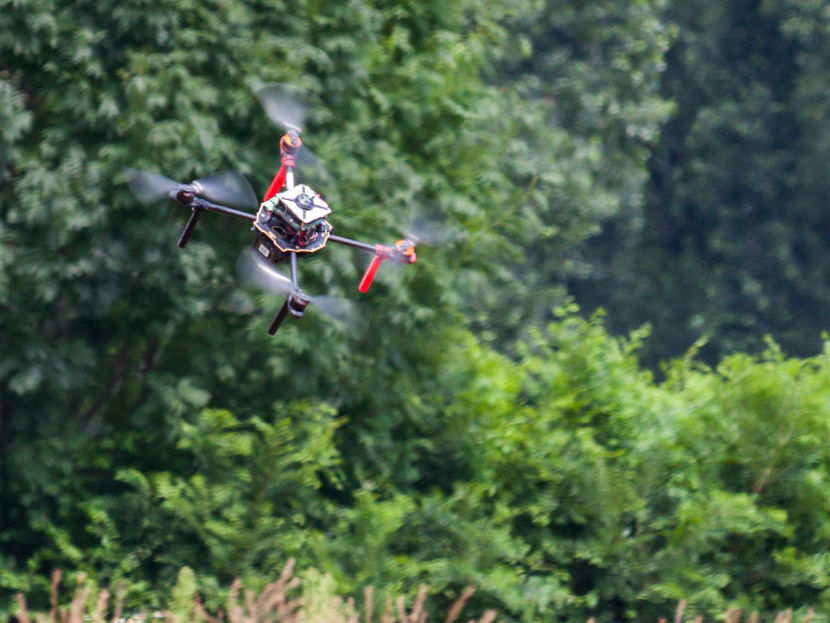
\includegraphics[width=0.30\textwidth]{./fig/photos/control_2_1-5.jpg}
  }
  \subfloat {
    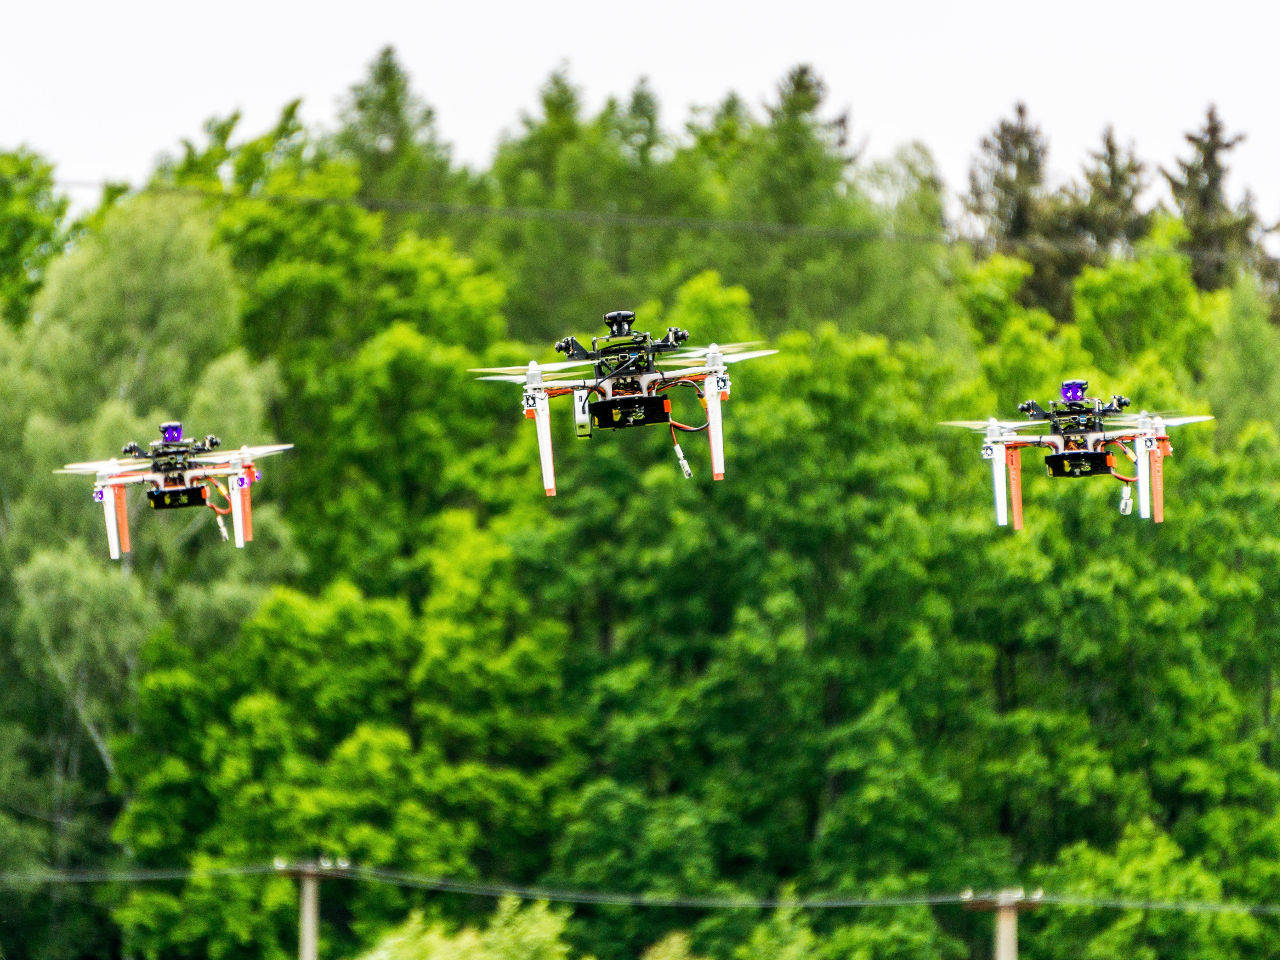
\includegraphics[width=0.30\textwidth]{./fig/photos/swarm_2_1-5.jpg}
  }
  \subfloat {
    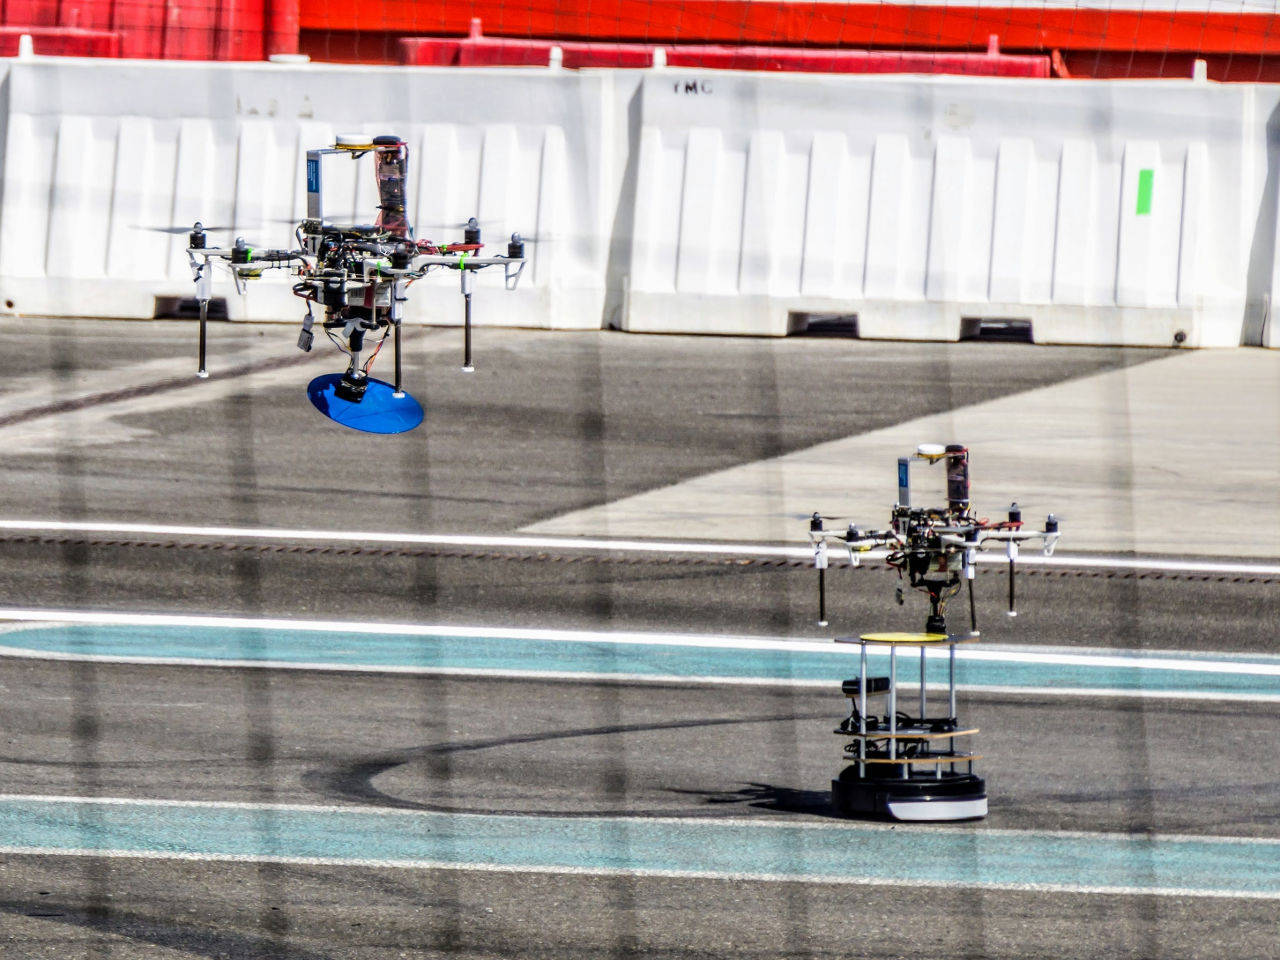
\includegraphics[width=0.30\textwidth]{./fig/photos/grasping_2017_2_1-5.jpg}
  }\\
  \vspace{-0.3em}
  \subfloat {
    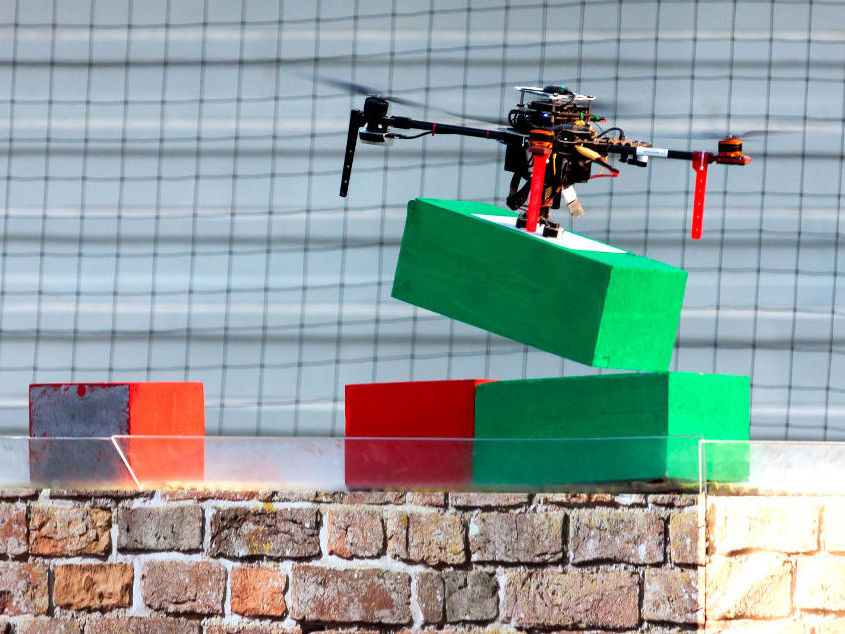
\includegraphics[width=0.30\textwidth]{./fig/photos/brick_placing_2_1-5.jpg}
  }
  \subfloat {
    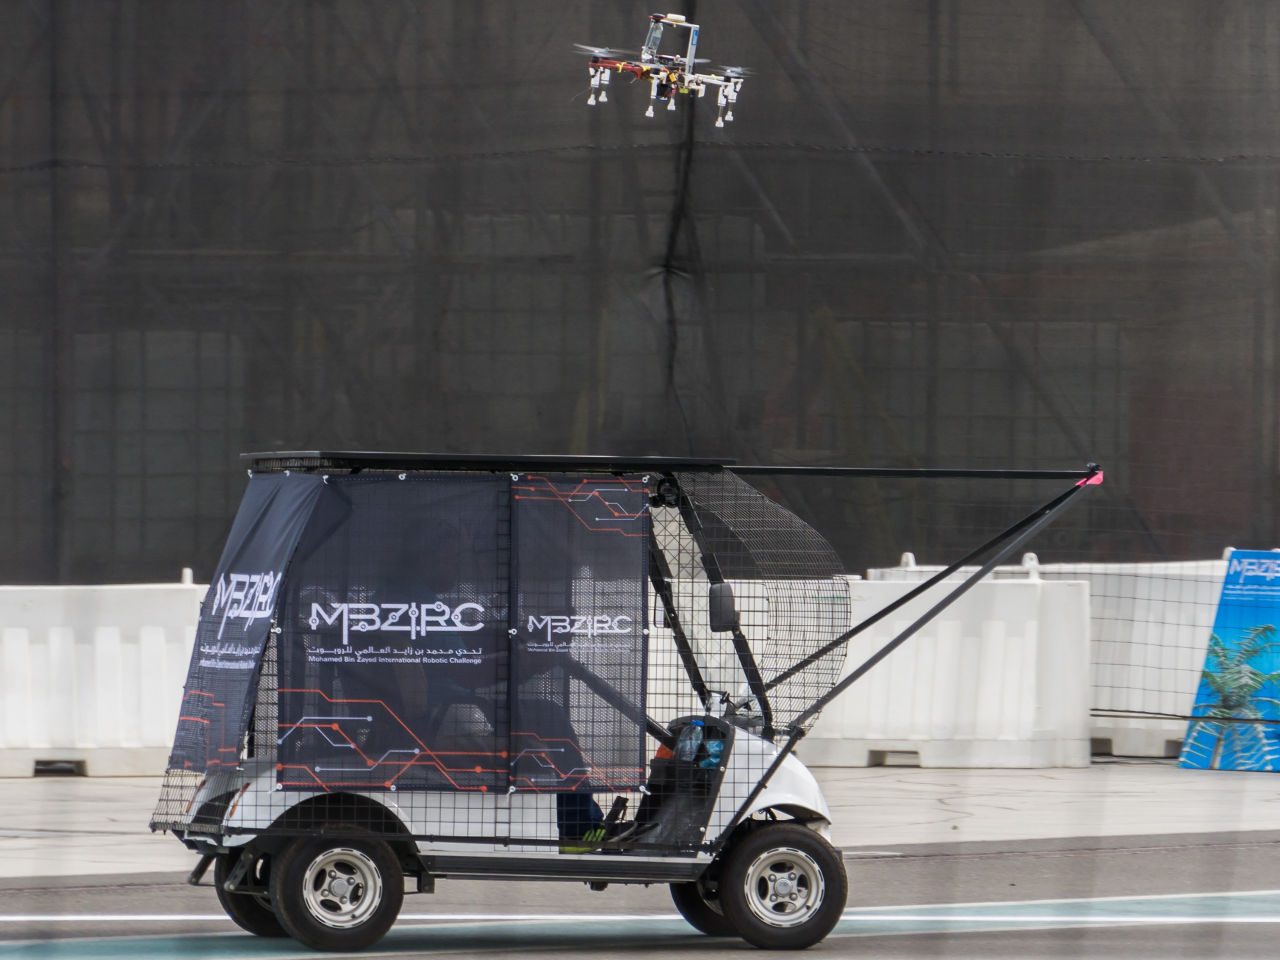
\includegraphics[width=0.30\textwidth]{./fig/photos/landing_2017_2_1-5.jpg}
  }
  \subfloat {
    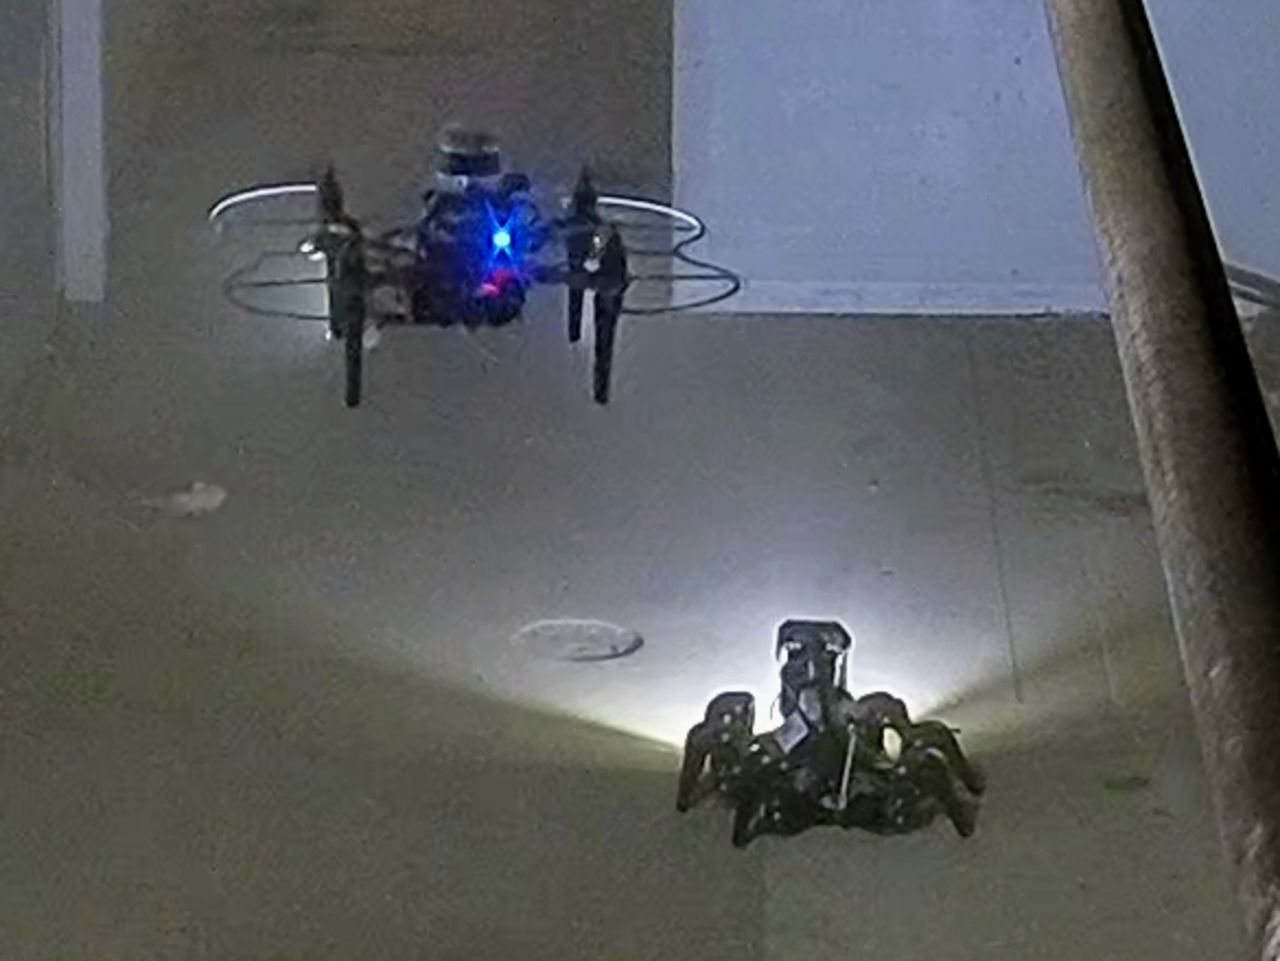
\includegraphics[width=0.30\textwidth]{./fig/photos/darpa_drone_beta_2_1-5.jpg}
  }\\
  \vspace{-0.3em}
  \subfloat {
    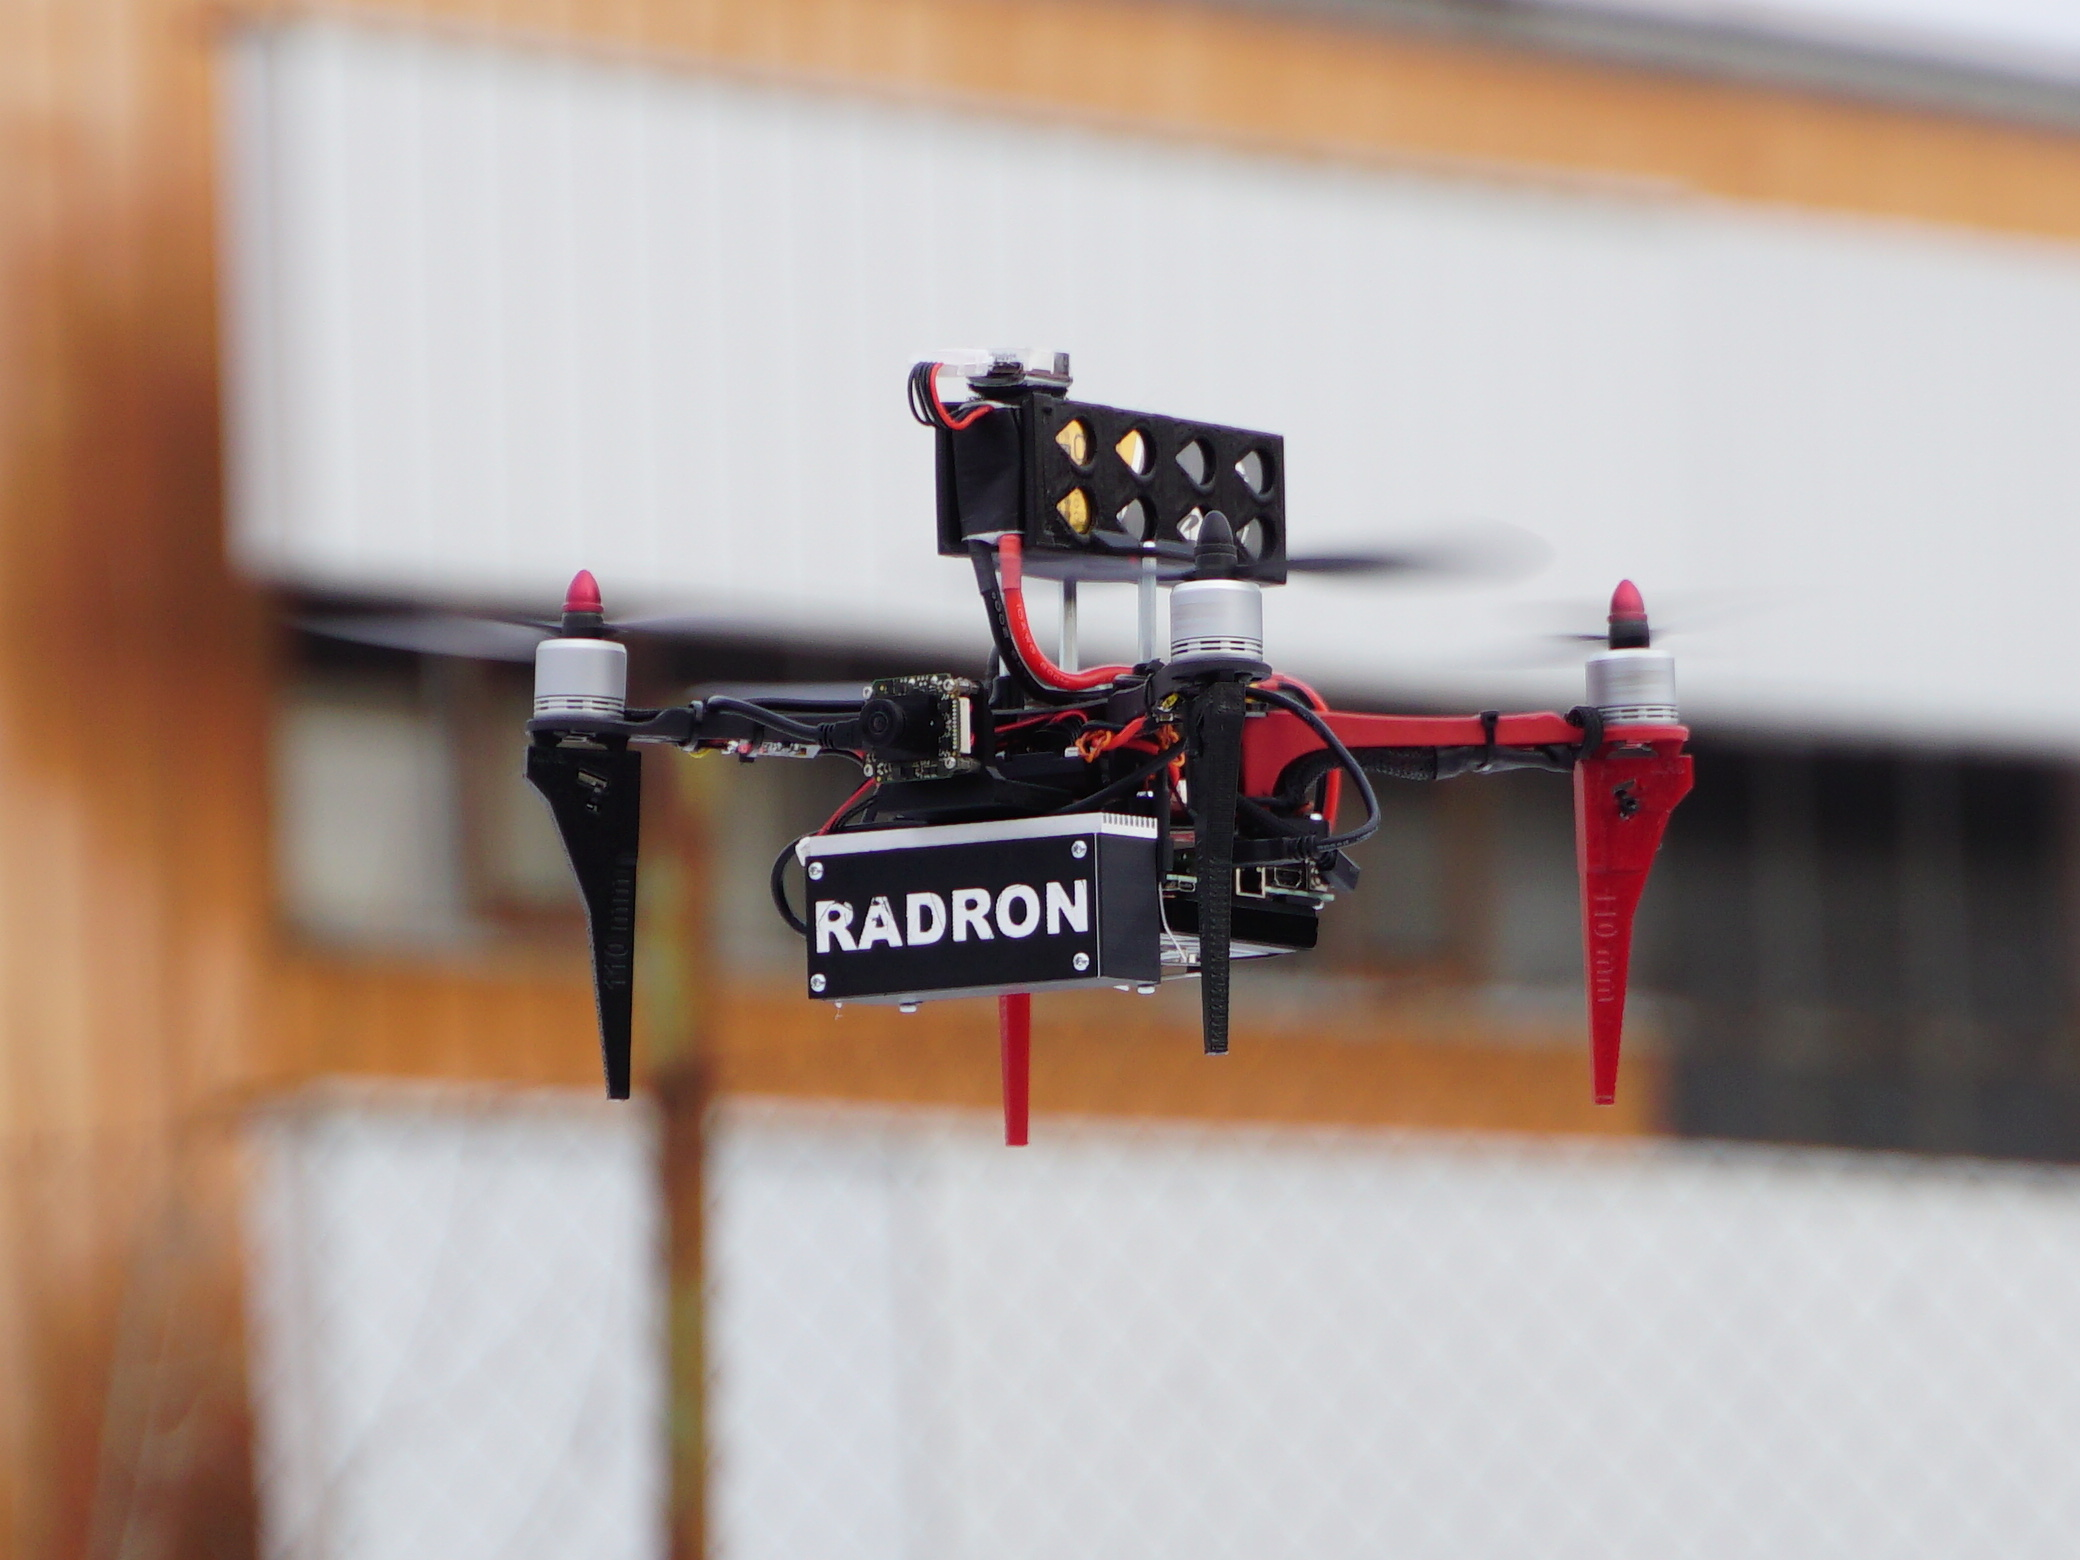
\includegraphics[width=0.30\textwidth]{./fig/photos/radron_vio_2_1-5.jpg}
  }
  \subfloat {
    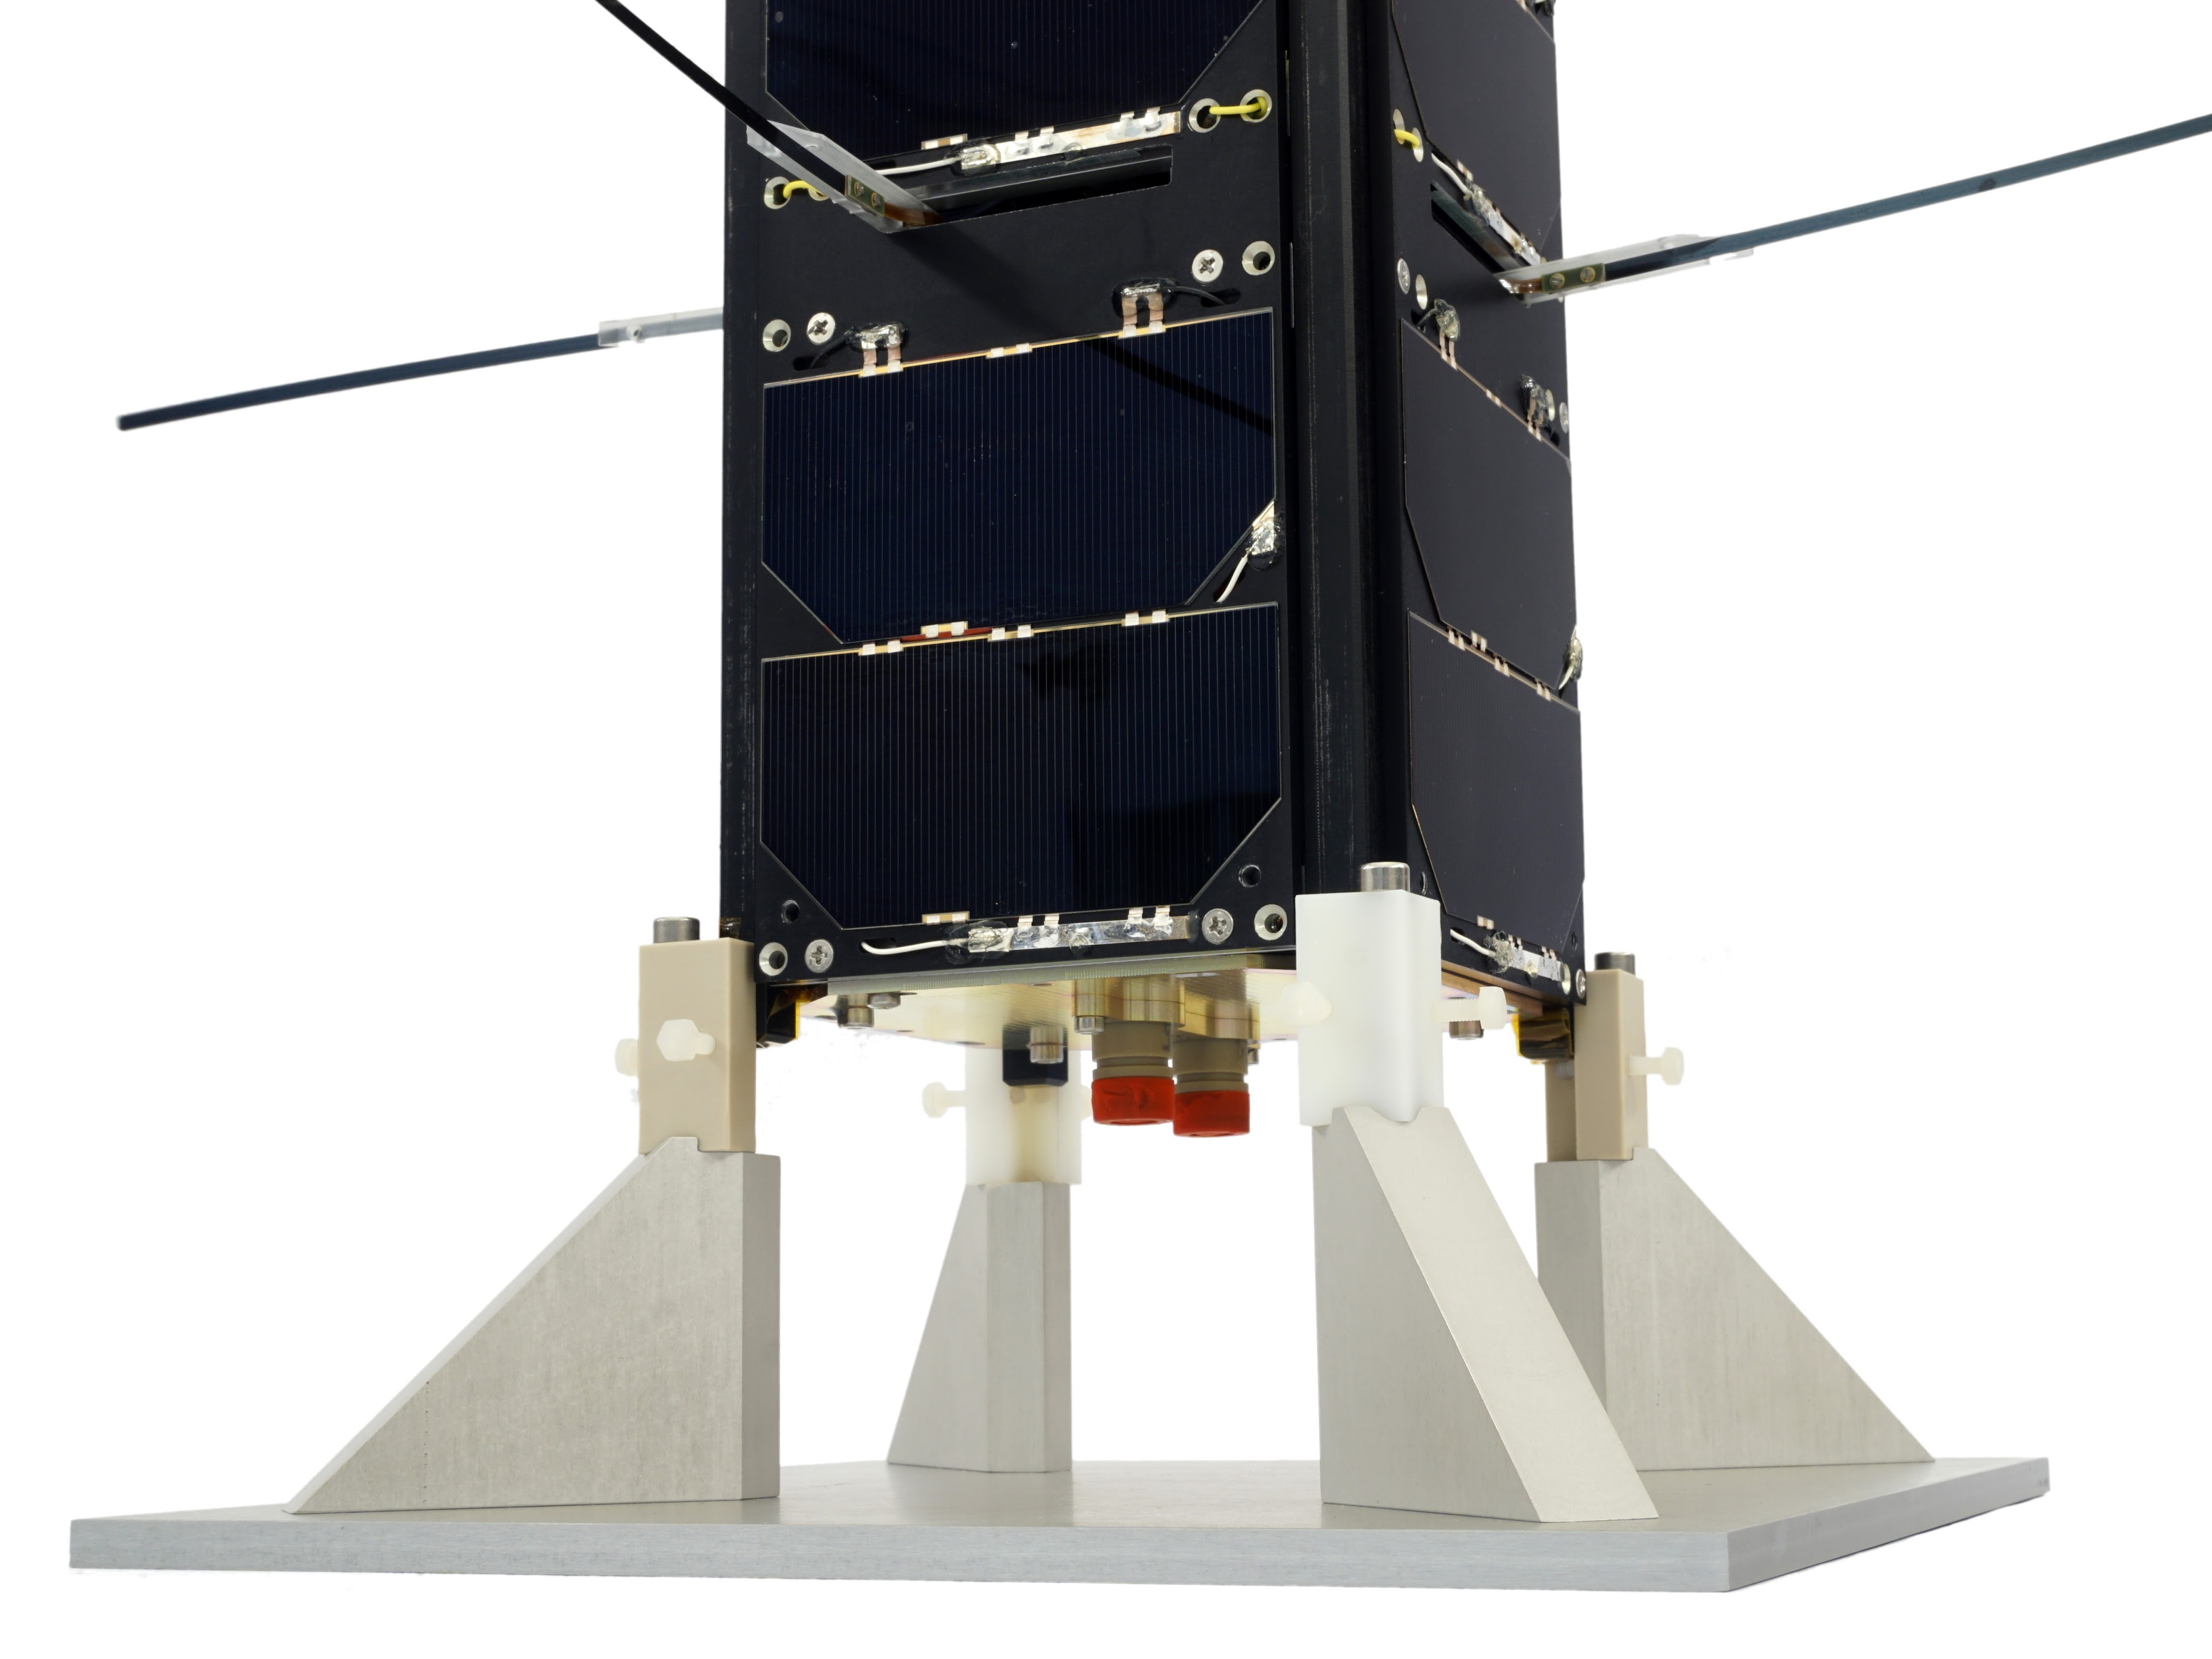
\includegraphics[width=0.30\textwidth]{./fig/photos/vzlusat_1_1-5.jpg}
  }
  \subfloat {
    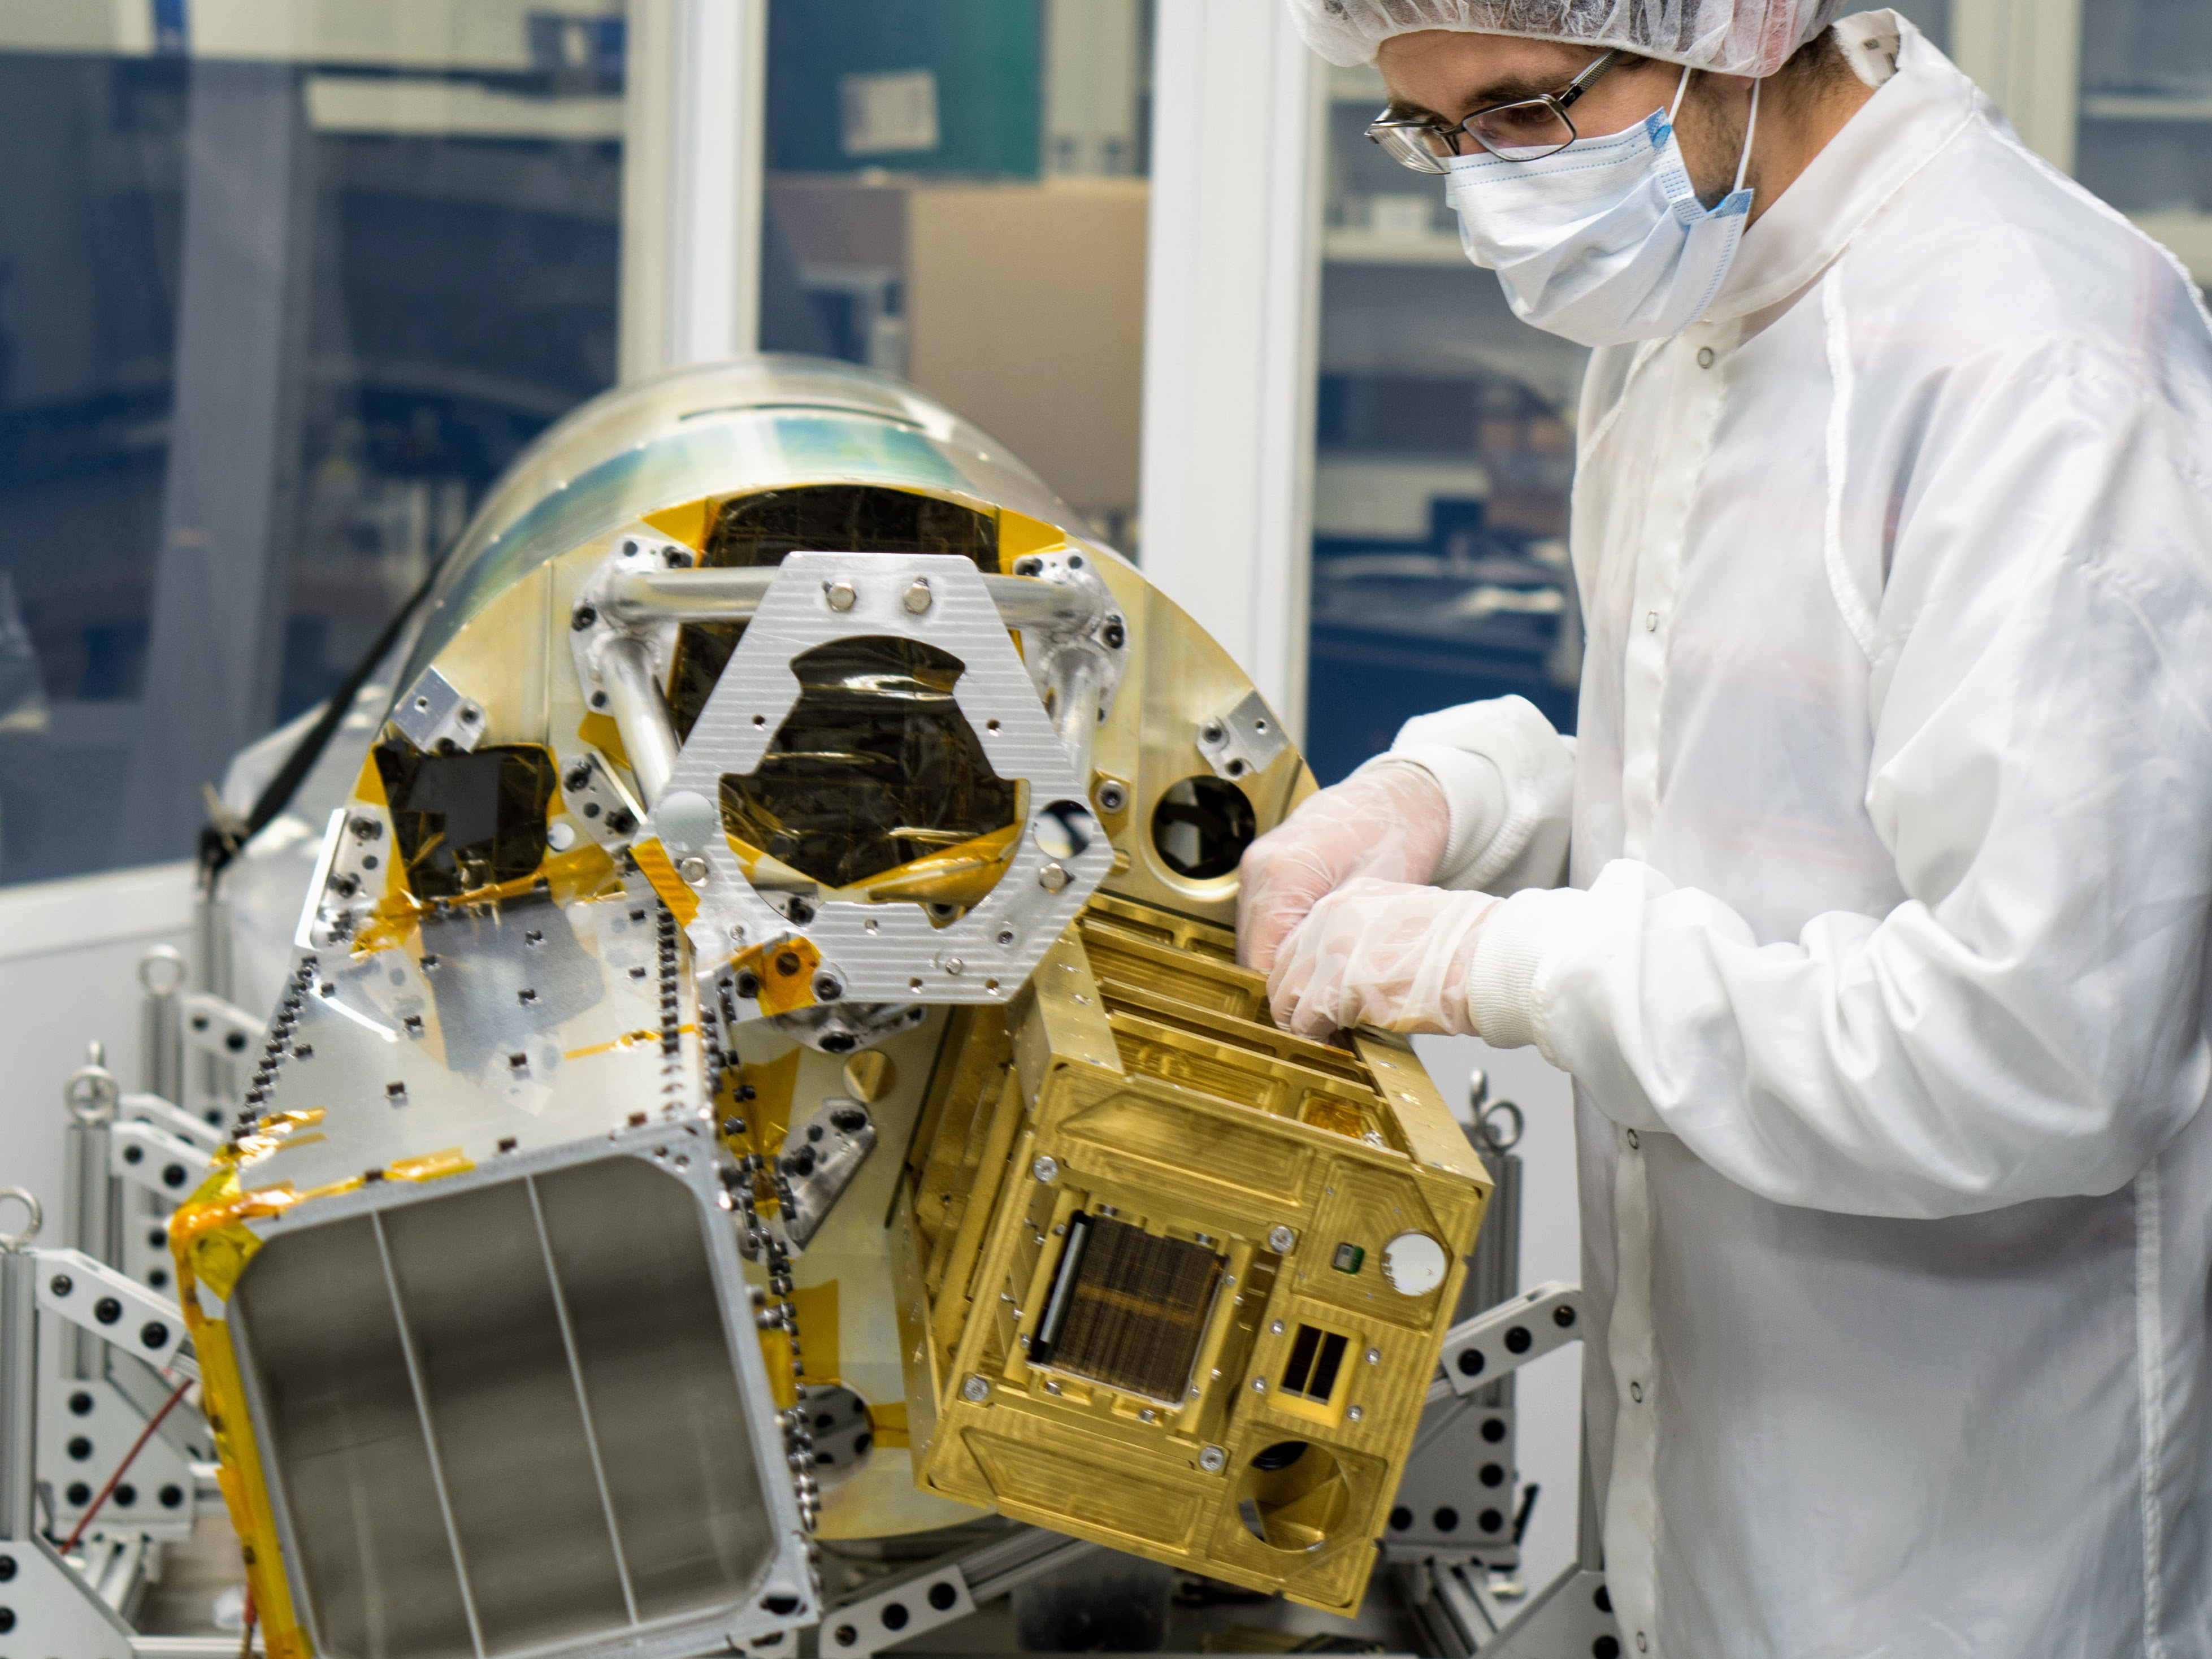
\includegraphics[width=0.30\textwidth]{./fig/photos/rex_1_1-5.jpg}
  }
  \caption{Illustration of outcomes of the thesis author's contributions: deployments of multi-rotor \acp{UAV} as well as radiation measurements for space applications.}
  \label{fig:collage}
\end{figure}

%%}

The objectives of the thesis are summarized as follows:

\textbf{(1) Development of a control system for real-world deployment of \acp{UAV}}, verification of new methods for control, remote sensing, and deployment in indoor and outdoor environments.
Despite many platforms for multirotor \acp{UAV} control and deployment are available, they lack features necessary for real-world testing and deployment of the methods within the focus of this thesis and the focus of the \acl{MRS} group at \ac{CTU} in Prague.
Therefore, the author's first objective and a long-term effort are to develop a modular \ac{UAV} control system.
The control system should allow safe indoor and outdoor deployment of multirotor helicopters.
The system should also allow verification of high-level methods for motion planning, multi-\ac{UAV} swarming, and formation flying.
Finally, the system should also allow basic research on low-level control and stabilization of the multirotor \ac{UAV} dynamics.

\textbf{(2) Research of methods of collaborative remote sensing} by a group of \aclp{UAV} in real-world non-laboratory conditions.
Collaboratively executing UAV missions poses challenges on many onboard autonomy levels, e.g., task allocation, estimation, motion planning, and control.
Furthermore, mutual communication between the \acp{UAV} might be unreliable or completely unavailable.
Therefore, sharing real-time sensor readings to pursue a common goal might not be possible in all circumstances.
Moreover, mutual collisions between the \acp{UAV} can be expected if the \acp{UAV} are guided by common goals.
The objective is to explore and push the field of collaborative remote sensing and deployment of \ac{UAV} in complex robotics tasks forwards.

\textbf{(3) Advancing the field of ionizing radiation dosimetry, mapping, and localization of compact sources} by \aclp{UAV}.
Ionizing radiation has been traditionally measured onboard \acp{UAV} using dosimeters \cite{nagatani2013emergency, sanada2015aerial, towler2012radiation, jiang2016prototype} --- sensors measuring the intensity of incoming radiation.
Often, the intensity is utilized only to estimate the scalar field of radiation intensity.
Rarely, direction measurement can be obtained with an additional device, e.g., the optical collimator or a coded aperture.
However, those solutions are not well-suited for small \acp{UAV} due to the heavyweight of the sensor equipment.
This thesis aims to push the state-of-the-art by utilizing miniature semiconductor pixel detectors \cite{llopart2007timepix}, and novel event-based radiation detectors \cite{poikela2014timepix3} onboard \acp{MAV}.

The rest of the thesis is organized as follows.
This thesis is a compilation of 8 included core publications, referenced as 1c -- 8c.
Furthermore, the thesis is supported by additional related authored publications, referenced as 9c -- 42c.
Firstly, the state of the art is summarized in Chapter~\ref{chap:sota}.
Chapter~\ref{chap:uav_platform} introduces the publications related to the developed \ac{UAV} platform.
Chapter~\ref{chap:sensing} covers the publications related to the multi-\ac{UAV} sensing and deployment.
Finally, Chapter~\ref{chap:radiation} presents publications on radiation measurement, localization, and mapping.

%%}

%% | ------------------------ Chapter 2 ----------------------- |

%%{ Contributions and Related Work

\chapter{Contributions and Related Work\label{chap:sota}}

\section{Author's publications and contributions}

Figure~\ref{fig:research_graph} shows a publication graph composed of accepted peer-review publications and publications that have been submitted in the time of writing this thesis.
The publications are split into four main categories.
The first category, a \emph{Pre-Ph.D. research}, consists of publications based upon the research done before the author started the pursue of Ph.D. ($\leq 2015$).
Although, some of these were written and submitted during the author's Ph.D. studies.
The second category is the research stream \ac{UAV} platform development for research validation and reliable deployment of novel methods in control, navigation, formation flying, and swarming.
Thirdly, the largest group of the author's publications is from the field of multi-\ac{UAV} remote sensing, swarming, and deployment.
Lastly, the fourth category is researching ionizing radiation detection, mapping, and localization.
The author conducts an interdisciplinary transfer from the space-oriented physics field to unmanned vehicles such as multirotor helicopters.

%%{ Fig: research graph

\begin{figure}

  %%{ tikzset

  \tikzset{
    article/.style={
      rectangle,
      inner sep=0pt,
      draw=black,
      text=black,
      minimum height=3.5em,
      minimum width=6.7em,
      text width=6.7em,
    },
    related/.style={
      rectangle,
      dashed,
      inner sep=0pt,
      draw=black,
      text=black,
      minimum height=3.5em,
      minimum width=6.7em,
      text width=6.7em,
      text height=3.0em,
      align=center,
    },
    subarticle/.style={
      rectangle,
      inner sep=0pt,
      draw=black,
      text=black,
      fill=black!15,
      minimum height=3.5em,
      minimum width=6.7em,
      text width=6.7em,
    },
    subkeyarticle/.style={
      rectangle,
      inner sep=0pt,
      draw=black,
      line width=0.75mm,
      text=black,
      fill=black!15,
      minimum height=3.5em,
      minimum width=6.7em,
      text width=6.7em,
    },
    keyarticle/.style={
      rectangle,
      inner sep=2pt,
      draw=black,
      text=black,
      line width=0.75mm,
      minimum height=3.5em,
      minimum width=6.5em,
      text width=6.5em,
    },
    stream/.style={
      rectangle,
      inner sep=2pt,
      draw=black,
      text=black,
      line width=0.5mm,
      minimum height=3em,
      minimum width=8em,
      rounded corners=1em,
      font=\bfseries,
    },
    technology/.style={
      rectangle,
      inner sep=2pt,
      draw=black,
      text=black,
      line width=0.5mm,
      minimum height=3.5em,
      minimum width=6.5em,
      rounded corners=0.5em,
      align=left,
    },
    cite/.style={
      rectangle,
      inner sep=2pt,
      text=black,
      draw=black,
      % minimum height=1em,
      text centered,
      anchor=south east,
    },
    keycite/.style={
      rectangle,
      inner sep=2pt,
      text=black,
      draw=black,
      line width=0.5mm,
      % minimum height=1em,
      text centered,
      anchor=south east,
    },
  }

  %%}

  %%{ commands

  \newcommand{\stream}[3]{
    \node[stream, #1] (#2) {\scriptsize #3};
  }

  \newcommand{\technology}[3]{
    \node[technology, #1] (#2) {\tiny #3};
  }

  \newcommand{\keyarticle}[4]{
    \node[keyarticle, #1] (#2) {\scalebox{0.9}{\tiny #4}};
    \node[keycite] at (#2.south east) {\tiny #3};
  }

  \newcommand{\article}[4]{
    \node[article, #1] (#2) {\scalebox{0.9}{\tiny #4}\vspace{0.1em}};
    \node[cite] at (#2.south east) {\tiny #3};
  }

  \newcommand{\related}[3]{
    \node[related, #1] (#2) {\scalebox{0.9}{\tiny #3}};
  }

  \newcommand{\subarticle}[4]{
    \node[subarticle, #1] (#2) {\scalebox{0.9}{\tiny #4}\vspace{0.1em}};
    \node[cite] at (#2.south east) {\tiny #3};
  }

  \newcommand{\subkeyarticle}[4]{
    \node[subkeyarticle, #1] (#2) {\scalebox{0.9}{\tiny #4}\vspace{0.1em}};
    \node[keycite] at (#2.south east) {\tiny #3};
  }

  %%}

  \centering

  \begin{adjustbox}{width=1.00\textwidth}

  \begin{tikzpicture}[node distance=1.0em and 1.0em, auto]

    %%{ block type headlines

    \stream{}{stream_generic}{Research stream}

    \technology{right=of stream_generic}{technology_generic}{
      \begin{tabular}{l}
        Key technology\\
        developped by\\
        the thesis author
      \end{tabular}
    }

    \keyarticle{right=of technology_generic}{keyarticle_generic}{1c}{
      \begin{tabular}{l}
        Key article\\
        included in\\
        the thesis
      \end{tabular}
    }

    \article{right=of keyarticle_generic}{article_generic}{1a}{
      \begin{tabular}{l}
        Authored article
      \end{tabular}
    }

    \subarticle{right=of article_generic}{subarticle_generic}{2a}{
      \begin{tabular}{l}
        Submitted article
      \end{tabular}
    }

    \related{right=of subarticle_generic}{dashedbox_generic}{
      Related articles
    }

    %%}

    %%{ precursor publications

    \article{below=of stream_generic,shift={(2.0em, -2em)}}{saska2013adhoc}{\tabcite{saska2013adhoc}}{
      \begin{tabular}{l}
        UAV-\acs{UGV}\\
        formations unde\\
        relative localization\\
        \emph{IROS 2013}
      \end{tabular}
    }

    \article{right=of saska2013adhoc}{chudoba2014localization}{\tabcite{chudoba2014localization}}{
      \begin{tabular}{l}
        UAV localization\\
        and stabilization\\
        using visual features\\
        \emph{ICUAS 2014}
      \end{tabular}
    }

    \article{right=of chudoba2014localization}{baca2016embedded}{\tabcite{baca2016embedded}}{
      \begin{tabular}{l}
        Embedded MPC\\
        for UAV control\\
        \emph{MMAR 2016}
      \end{tabular}
    }

    \article{right=of baca2016embedded}{saska2017documentation}{\tabcite{saska2017documentation}}{
      \begin{tabular}{l}
        Documentation of\\
        historical buildings\\
        using UAVs\\
        \emph{ETFA 2017}
      \end{tabular}
    }

    \article{below=of saska2013adhoc,shift={(0em, 0em)}}{chudoba2016exploration}{\tabcite{chudoba2016exploration}}{
      \begin{tabular}{l}
        Exploration for\\
        visual feature-based\\
        UAV navigation\\
        \emph{JIRS 2016}
      \end{tabular}
    }

    \article{right=of chudoba2016exploration}{saska2016formations}{\tabcite{saska2016formations}}{
      \begin{tabular}{l}
        UAV formations\\
        with migrating\\
        virtual leader\\
        \emph{ICARCV 2016}
      \end{tabular}
    }

    \article{right=of saska2016formations}{spurny2016complex}{\tabcite{spurny2016complex}}{
      \begin{tabular}{l}
        Complex manouvres\\
        of UAV-UGV\\
        formations\\
        \emph{MMAR 2016}
      \end{tabular}
    }

    \article{right=of spurny2016complex}{saska2017system}{\tabcite{saska2017system}}{
      \begin{tabular}{l}
        System for UAV\\
        in GPS-denied\\
        environments\\
        \emph{AuRo 2017}
      \end{tabular}
    }

    \article{right=of baca2016embedded, shift={(10.5em, 0.0em)}}{baca2016miniaturized}{\tabcite{baca2016miniaturized}}{
      \begin{tabular}{l}
        X-Ray telescope\\
        with Timepix sensor\\
        for VZLUSAT-1\\
        nanosatellite\\
        \emph{JINST 2016}
      \end{tabular}
    }

    \article{below=of baca2016miniaturized}{daniel2016terrestrial}{\tabcite{daniel2016terrestrial}}{
      \begin{tabular}{l}
        Terrestrial gamma\\
        ray monitor on\\
        a cubesat\\
        \emph{SPIE O\&P 2016}\\
      \end{tabular}
    }

    %%}

    %%{ research stream headlines

    \stream{below=of stream_generic, shift={(0.00em, -11.5em)}}{uav_platform_stream}{
      \begin{tabular}{l}
        UAV platform\\
        for research
      \end{tabular}
    }

    \stream{right=of uav_platform_stream}{uav_sensing_stream}{
      \hspace{5em}
      \begin{tabular}{l}
        UAVs in remote sensing,\\
        data gathering and swarming
      \end{tabular}
      \hspace{5em}
    }

    \stream{right=of uav_sensing_stream}{radiation_stream}{
      \hspace{3em}
      \begin{tabular}{l}
        Ionizing Radiation\\
        dosimetry and imaging
      \end{tabular}
      \hspace{3em}
    }

    \node [rotate=90, left=of stream_generic, shift={(-4.2em, -1.5em)}] {Pre-Ph.D. research};

    %%}

    %%{ blocks

    \keyarticle{below=of radiation_stream,shift={(-4em, 0)}}{baca2018timepix}{\tabcite{baca2018timepix}}{
      \begin{tabular}{l}
        1 year of\\
        VZLUSAT-1\\
        dosimetry in orbit\\
        \emph{JINST 2018}
      \end{tabular}
    }

    \article{right=of baca2018timepix}{urban2017vzlusat}{\tabcite{urban2017vzlusat}}{
      \begin{tabular}{l}
        VZLUSAT-1\\
        nanosatellite\\
        \emph{AA 2017}
      \end{tabular}
    }

    \article{below=of urban2017vzlusat}{daniel2019inorbit}{\tabcite{daniel2019inorbit}}{
      \begin{tabular}{l}
        Commissioning\\
        of VZLUSAT-1\\
        nanosatellite\\
        \emph{SSR 2019}
      \end{tabular}
    }

    \technology{below=of baca2018timepix}{rospix_technology}{
      \begin{tabular}{l}
        Rospix: Timepix\\
        controller\\
        for ROS
      \end{tabular}
    }

    \technology{below=of uav_platform_stream}{mpc_tracker_technology}{
      \begin{tabular}{l}
        MPC Tracker for\\
        UAV trajectory\\
        following
      \end{tabular}
    }

    \article{below=of uav_sensing_stream,shift={(-4em, 0em)}}{loianno2018localization}{\tabcite{loianno2018localization}}{
      \begin{tabular}{l}
        Localization of\\
        objects by UAVs\\
        \emph{RA-L 2018}
      \end{tabular}
    }

    \keyarticle{right=of loianno2018localization}{spurny2019cooperative}{\tabcite{spurny2019cooperative}}{
      \begin{tabular}{l}
        Cooperative object\\
        gathering by UAVs\\
        \emph{JFR 2019}
      \end{tabular}
    }

    \article{below=of loianno2018localization,shift={(0em, 0em)}}{baca2017autonomous}{\tabcite{baca2017autonomous}}{
      \begin{tabular}{l}
        Autonomous UAV\\
        landing on a car\\
        \emph{ECMR 2017}
      \end{tabular}
    }

    \keyarticle{right=of baca2017autonomous}{baca2019autonomous}{\tabcite{baca2019autonomous}}{
      \begin{tabular}{l}
        Autonomous UAV\\
        landing on a car\\
        \emph{JFR 2019}
      \end{tabular}
    }

    \article{below=of $(rospix_technology.south |- baca2019autonomous.south)$,shift={(0em, -1em)}}{baca2018rospix}{\tabcite{baca2018rospix}}{
      \begin{tabular}{l}
        Rospix: Timepix\\
        interface for Robot\\
        Operating System\\
        \emph{JINST 2018}
      \end{tabular}
    }

    \article{right=of baca2018rospix}{daniel2017xray}{\tabcite{daniel2017xray}}{
      \begin{tabular}{l}
        X-Ray telescope\\
        for a sounding\\
        rocket experiment\\
        \emph{SPIE O\&P 2017}
      \end{tabular}
    }

    \keyarticle{below=of $(mpc_tracker_technology.south |- loianno2018localization.south)$}{baca2018model}{\tabcite{baca2018model}}{
      \begin{tabular}{l}
        Model Predictive\\
        Control Tracker\\
        for UAVs\\
        \emph{IROS 2018}
      \end{tabular}
    }

    \technology{below=of $(baca2018model.south |- baca2017autonomous.south)$,shift={(0em, -1em)}}{mrs_uav_system_technology}{
      \begin{tabular}{l}
        MRS UAV System
      \end{tabular}
    }

    \article{below=of baca2017autonomous.south,shift={(0em, -1em)}}{faigl2017onsolution}{\tabcite{faigl2017onsolution}}{
      \begin{tabular}{l}
        On solution of\\
        Dubins touring\\
        problem\\
        \emph{ECMR 2017}
      \end{tabular}
    }

    \article{below=of $(mrs_uav_system_technology.south |- faigl2017onsolution.south)$}{petrlik2020robust}{\tabcite{petrlik2020robust}}{
      \begin{tabular}{l}
        Robust UAV system\\
        for constrained\\
        environment\\
        \emph{RA-L 2020}
      \end{tabular}
    }

    \article{below=of faigl2017onsolution,shift={(0em, 0em)}}{roucek2019darpa}{\tabcite{roucek2019darpa}}{
      \begin{tabular}{l}
        DARPA SubT\\
        mine exploration\\
        by Robots\\
        \emph{MESAS 2019}
      \end{tabular}
    }

    \subarticle{right=of roucek2019darpa,shift={(0.0em, 0.0em)}}{kratky2020autonomous2}{\tabcite{kratky2020autonomous2}}{
      \begin{tabular}{l}
        DARPA SubT\\
        Urban exploration\\
        \emph{JFR 2020}
      \end{tabular}
    }

    \article{below=of roucek2019darpa,shift={(0em, 0em)}}{saikin2020wildfire}{\tabcite{saikin2020wildfire}}{
      \begin{tabular}{l}
        Wildlife firefighting\\
        with UAVs\\
        \emph{RA-L 2020}
      \end{tabular}
    }

    \subarticle{right=of saikin2020wildfire,shift={(0em, 0em)}}{silano2020power}{\tabcite{silano2020power}}{
      \begin{tabular}{l}
        Powerline inspection\\
        with UAVs using\\
        STL\\
        \emph{RA-L 2020}
      \end{tabular}
    }

    \article{right=of faigl2017onsolution,shift={(0em, 0em)}}{giernacki2019realtime}{\tabcite{giernacki2019realtime}}{
      \begin{tabular}{l}
        Real-time UAV\\
        controller tuning\\
        \emph{Sensors 2019}
      \end{tabular}
    }

    \article{below=of saikin2020wildfire,shift={(0em, 0em)}}{petracek2020bioinspired}{\tabcite{petracek2020bioinspired}}{
      \begin{tabular}{l}
        Bio-inspired\\
        compact UAV\\
        swarms\\
        \emph{B\&B 2020}\\
      \end{tabular}
    }

    \subkeyarticle{below=of $(petrlik2020robust.south |- petracek2020bioinspired.south)$,shift={(0em, 0em)}}{baca2020mrs}{\tabcite{baca2020mrs}}{
      \begin{tabular}{l}
        MRS UAV system\\
        for research\\
        evaluation\\
        \emph{JINT 2020}
      \end{tabular}
    }

    \article{right=of petracek2020bioinspired,shift={(0em, 0em)}}{saska2020formation}{\tabcite{saska2020formation}}{
      \begin{tabular}{l}
        Formations of UAVs\\
        straitened\\
        environments\\
        \emph{AuRo, 2020}\\
      \end{tabular}
    }

    \subarticle{below=of $(daniel2017xray.south |- saska2020formation.south)$}{urban2020rex}{\tabcite{urban2020rex}}{
      \begin{tabular}{l}
        X-Ray telescope\\
        on NASA's sounding\\
        rocket experiment\\
        \emph{AA 2020}
      \end{tabular}
    }

    \subarticle{below=of petracek2020bioinspired,shift={(0em, 0em)}}{ahmad2020autonomous}{\tabcite{ahmad2020autonomous}}{
      \begin{tabular}{l}
        Autonomous UAV\\
        swarms without\\
        \acs{GNSS} and comm.\\
        \emph{ICRA, 2021}\\
      \end{tabular}
    }

    \subarticle{right=of ahmad2020autonomous,shift={(0em, 0em)}}{dmytruk2020safe}{\tabcite{dmytruk2020safe}}{
      \begin{tabular}{l}
        Tightly-constrained\\
        UAV swarms\\
        without GNSS\\
        \emph{ICRA, 2021}\\
      \end{tabular}
    }

    \keyarticle{below=of $(baca2018rospix.south |- faigl2017onsolution.south)$,shift={(-4.6em, 0.0em)}}{baca2019timepix}{\tabcite{baca2019timepix}}{
      \begin{tabular}{l}
        Radiation mapping\\
        with Timepix sensor\\
        onboard UAV\\
        \emph{IROS 2019}
      \end{tabular}
    }

    \keyarticle{below=of baca2019timepix,shift={(0.0em, 0em)}}{stibinger2020localization}{\tabcite{stibinger2020localization}}{
      \begin{tabular}{l}
        Radiation mapping\\
        with Timepix sensor\\
        by UAVs\\
        \emph{RA-L 2020}
      \end{tabular}
    }

    \subarticle{below=of $(stibinger2020localization.south |- saska2020formation.south)$}{baca2020gamma}{\tabcite{baca2020gamma}}{
      \begin{tabular}{l}
        $\gamma$-source localization\\
        by a UAV with\\
        a Compton camera\\
        \emph{ICRA 2020}
      \end{tabular}
    }

    \subarticle{below=of $(ahmad2020autonomous.south |- baca2020mrs.south)$,shift={(-4.0em, -1.0em)}}{walter2020extinguishing}{\tabcite{walter2020extinguishing}}{
      \begin{tabular}{l}
        Extinguishing of\\
        ground fires\\
        by UAVs\\
        \emph{ICRA, 2021}
      \end{tabular}
    }

    \subarticle{right=of walter2020extinguishing,shift={(0.0em, -0em)}}{stasinchuk2020multiuav}{\tabcite{stasinchuk2020multiuav}}{
      \begin{tabular}{l}
        Autonomous\\
        target elimination\\
        by UAVs\\
        \emph{ICRA, 2021}
      \end{tabular}
    }

    \subarticle{below=of baca2020mrs,shift={(0.0em, -1em)}}{smrcka2020admittance}{\tabcite{smrcka2020admittance}}{
      \begin{tabular}{l}
        Admittance UAV\\
        stabilization for\\
        building inspection\\
        \emph{ICRA, 2021}
      \end{tabular}
    }

    \subarticle{right=of stasinchuk2020multiuav,shift={(0.0em, -0em)}}{spurny2020autonomous}{\tabcite{spurny2020autonomous}}{
      \begin{tabular}{l}
        Autonomous UAV\\
        firefighting inside\\
        a building\\
        \emph{IEEE Access, 2020}
      \end{tabular}
    }

    \subarticle{below=of walter2020extinguishing,shift={(0.0em, -0em)}}{vrba2020autonomous}{\tabcite{vrba2020autonomous}}{
      \begin{tabular}{l}
        Autonomous target\\
        capturing by a UAV\\
        \emph{SMCA 2020}
      \end{tabular}
    }

    \subkeyarticle{right=of vrba2020autonomous,shift={(0.0em, -0em)}}{baca2020autonomous}{\tabcite{baca2020autonomous}}{
      \begin{tabular}{l}
        Autonomous wall\\
        building by a group\\
        of UAVs\\
        \emph{RAS 2020}
      \end{tabular}
    }

    %%}

    %%{ backgrounds

    \begin{pgfonlayer}{background}
      \path (spurny2019cooperative.east |- spurny2019cooperative.north)+(+0.2, 0.2) node (a) {};
      \path (baca2017autonomous.south -| baca2017autonomous.west)+(-0.2,-0.4) node (b) {};
      \path[fill=black!0, draw=black!50, dashed]
      (a) rectangle (b);
      \path ($(a |- b)$) -- node [midway, shift = {(0.0, 1.5em)}] {\begin{tabular}{c}
        \tiny MBZIRC 2017\\
      \end{tabular}} ($(b |- b)$);
    \end{pgfonlayer}

    \begin{pgfonlayer}{background}
      \path (spurny2020autonomous.east |- spurny2020autonomous.north)+(+0.2, 0.2) node (a) {};
      \path (vrba2020autonomous.south -| vrba2020autonomous.west)+(-0.2,-0.4) node (b) {};
      \path[fill=black!00, draw=black!50, dashed]
      (a) rectangle (b);
      \path ($(a |- b)$) -- node [midway, shift = {(0.0, 1.5em)}] {\begin{tabular}{c}
        \tiny MBZIRC 2020\\
      \end{tabular}} ($(b |- b)$);
    \end{pgfonlayer}

    \begin{pgfonlayer}{background}
      \path (saska2020formation.east |- saska2020formation.north)+(+0.2, 0.2) node (a) {};
      \path (ahmad2020autonomous.south -| ahmad2020autonomous.west)+(-0.2,-0.4) node (b) {};
      \path[fill=black!00, draw=black!50, dashed]
      (a) rectangle (b);
      \path ($(a |- b)$) -- node [midway, shift = {(0.0, 1.5em)}] {\begin{tabular}{c}
        \tiny UAV Formations and Swarms\\
      \end{tabular}} ($(b |- b)$);
    \end{pgfonlayer}

    %%}

  %%{ paths

    \path[-] (baca2016miniaturized) edge [->] (daniel2016terrestrial);

    \path[-] (baca2018timepix) edge [->] (rospix_technology);
    \path[-] (rospix_technology) edge [->] (baca2018rospix);
    \path[-] (baca2018timepix) edge [->] (urban2017vzlusat);
    \path[-] (urban2017vzlusat) edge [->] (daniel2019inorbit);

    \path[-] (loianno2018localization) edge [->] (spurny2019cooperative);
    \path[-] (baca2017autonomous) edge [->] (baca2019autonomous);

    \path[-] (daniel2017xray) edge [->] (urban2020rex);

    \draw[-] ($(baca2016miniaturized.west)$) -- ($(radiation_stream.north |- baca2016miniaturized.east) + (-5.75em, 0.0em)$) edge [->] ($(radiation_stream.north) + (-5.75em, 0.0em)$);

    \path[-] (saska2013adhoc) edge [->] (chudoba2014localization);
    \path[-] (chudoba2014localization) edge [->] (baca2016embedded);
    \path[-] (baca2016embedded) edge [->] (saska2017documentation);
    \draw[-] ($(baca2016embedded.south)$) -- ($(baca2016embedded.south) + (0, -0.5em)$) -- ($(chudoba2016exploration.north |-baca2016embedded.south) + (0, -0.5em)$) edge [->] (chudoba2016exploration.north);
    \draw[-] ($(baca2016embedded.south)$) -- ($(baca2016embedded.south) + (0, -0.5em)$) -- ($(uav_platform_stream.north |-baca2016embedded.south) + (-2.0em, -0.5em)$) edge [->] ($(uav_platform_stream.north) + (-2.0em, 0em)$);
    \draw[-] ($(baca2016embedded.south)$) -- ($(baca2016embedded.south) + (0, -0.5em)$) -- ($(saska2016formations.north |-baca2016embedded.south) + (0, -0.5em)$) edge [->] (saska2016formations.north);
    \draw[-] ($(baca2016embedded.south)$) -- ($(baca2016embedded.south) + (0, -0.5em)$) -- ($(spurny2016complex.north |-baca2016embedded.south) + (0, -0.5em)$) edge [->] (spurny2016complex.north);
    \draw[-] ($(baca2016embedded.south)$) -- ($(baca2016embedded.south) + (0, -0.5em)$) -- ($(saska2017system.north |-baca2016embedded.south) + (0, -0.5em)$) edge [->] (saska2017system.north);

    \draw[-] ($(chudoba2016exploration.south)$) -- ($(chudoba2016exploration.south) + (0, -0.5em)$) -- ($(uav_sensing_stream.north |-chudoba2016exploration.south) + (0, -0.5em)$) edge [->] (uav_sensing_stream.north);
    \draw[-] ($(saska2016formations.south)$) -- ($(saska2016formations.south) + (0, -0.5em)$) -- ($(uav_sensing_stream.north |-saska2016formations.south) + (0, -0.5em)$) edge [->] (uav_sensing_stream.north);
    \draw[-] ($(spurny2016complex.south)$) -- ($(spurny2016complex.south) + (0, -0.5em)$) -- ($(uav_sensing_stream.north |-spurny2016complex.south) + (0, -0.5em)$) edge [->] (uav_sensing_stream.north);
    \draw[-] ($(saska2017system.south)$) -- ($(saska2017system.south) + (0, -0.5em)$) -- ($(uav_sensing_stream.north |-saska2017system.south) + (0, -0.5em)$) edge [->] (uav_sensing_stream.north);

    \draw[<-] ($(mrs_uav_system_technology.east)$) -- ($(mrs_uav_system_technology.east) + (2.2em, 0.0em)$) -- ($(mrs_uav_system_technology.east) + (2.2em, 0.0em)$) edge [->] ($(mrs_uav_system_technology.east |- stasinchuk2020multiuav.north) + (2.2em, 0.6em)$);
    \draw[-] ($(mrs_uav_system_technology.east)$) -- ($(mrs_uav_system_technology.east) + (2.2em, 0.0em)$) -- ($(mrs_uav_system_technology.east) + (2.2em, 0.0em)$) -- ($(mrs_uav_system_technology.east |- saikin2020wildfire.west) + (2.2em, 0.0em)$) edge [->] ($(saikin2020wildfire.west) + (0.0em, 0.0em)$);
    \draw[-] ($(mrs_uav_system_technology.east)$) -- ($(mrs_uav_system_technology.east) + (2.2em, 0.0em)$) -- ($(mrs_uav_system_technology.east) + (2.2em, 0.0em)$) -- ($(mrs_uav_system_technology.east |- petracek2020bioinspired.west) + (2.2em, 0.0em)$) edge [->] ($(petracek2020bioinspired.west) + (-0.6em, 0.0em)$);
    \draw[-] ($(mrs_uav_system_technology.east)$) -- ($(mrs_uav_system_technology.east) + (2.2em, 0.0em)$) -- ($(mrs_uav_system_technology.east) + (2.2em, 0.0em)$) -- ($(mrs_uav_system_technology.east |- smrcka2020admittance.north) + (2.2em, 1.2em)$) -- ($(smrcka2020admittance.north) + (0.0em, 1.2em)$) edge [->] ($(smrcka2020admittance.north) + (0.0em, 0.0em)$);
    \draw[-] ($(mrs_uav_system_technology.east)$) -- ($(mrs_uav_system_technology.east) + (2.2em, 0.0em)$) -- ($(mrs_uav_system_technology.east |- giernacki2019realtime.south) + (2.2em, -0.5em)$) -- ($(giernacki2019realtime.south) + (0.0em, -0.5em)$) edge [->] ($(giernacki2019realtime.south) + (0.0em, 0.0em)$);
    \draw[-] ($(mrs_uav_system_technology.east)$) -- ($(mrs_uav_system_technology.east) + (2.2em, 0.0em)$) -- ($(mrs_uav_system_technology.east |- silano2020power.north) + (2.2em, 0.5em)$) -- ($(silano2020power.north) + (0.0em, 0.5em)$) edge [->] ($(silano2020power.north) + (0.0em, 0.0em)$);

    \draw[-] ($(urban2017vzlusat.east)$) -- ($(urban2017vzlusat.east) + (1.0em, 0.0em)$) -- ($(urban2017vzlusat.east) + (1.0em, 0.0em)$) -- ($(urban2017vzlusat.east |- daniel2017xray.east) + (1.0em, 0.0em)$) edge [->] ($(daniel2017xray.east) + (0.0em, 0.0em)$);

    \draw[-] ($(rospix_technology.south)$) -- ($(rospix_technology.south) + (0, -0.5em)$) -- ($(baca2019timepix.north |-rospix_technology.south) + (0, -0.5em)$) edge [->] (baca2019timepix.north);

    \path[-] (baca2019timepix) edge [->] (stibinger2020localization);
    \path[-] (mrs_uav_system_technology.east) edge [<->] ($(faigl2017onsolution.west |- mrs_uav_system_technology.east)$);
    \path[-] (roucek2019darpa) edge [->] (kratky2020autonomous2);
    \path[-] (petrlik2020robust.east) edge [<->] (roucek2019darpa.west);

    \draw[-] ($(rospix_technology.east) + (0.0em, 0.0em)$) -- ($(rospix_technology.east) + (0.5em, 0.0em)$) -- ($(rospix_technology.east |- baca2020gamma.west) + (0.5em, 0.0em)$) edge [->] (baca2020gamma.east);
    \draw[-] ($(rospix_technology.east) + (0.0em, 0.0em)$) -- ($(rospix_technology.east) + (0.5em, 0.0em)$) -- ($(rospix_technology.east |- urban2020rex.west) + (0.5em, 0.0em)$) edge [->] (urban2020rex.west);

    \path[-] (mpc_tracker_technology) edge [->] (baca2018model);
    \path[-] (baca2018model) edge [->] (mrs_uav_system_technology);
    \path[-] (mrs_uav_system_technology) edge [->] (petrlik2020robust);
    \path[-] (petrlik2020robust) edge [->] (baca2020mrs);
    \path[-] (mpc_tracker_technology) edge [<->] ($(loianno2018localization.west |- mpc_tracker_technology.east) + (-0.6em, 0)$);

  %%}

  \end{tikzpicture}

  \end{adjustbox}

  \caption{
    Diagram of research performed by the thesis author from 2013 to 2020 in the fields of UAV control, remote sensing and its applications, and the field of ionizing radiation imaging, dosimetry, mapping and localization.
    The article numbering reflects the works in the reference section of this thesis.
  }

  \label{fig:research_graph}

\end{figure}

%%}

%%{ Multirotor UAV control system

\section{Multirotor UAV control system}

Commercial \ac{UAV} systems are often closed-source and provide features tailored for photographers, video makers, and hobby pilots.
Autonomous operation of commercial \acp{UAV} is typically limited to a single aerial vehicle flying outdoors under a \ac{GNSS} localization while following a set of waypoints.
Therefore, commercial platforms are rarely used for research.
If so, then in a field where the \ac{UAV} is only considered a \emph{sensor carrier}, without added onboard autonomy.

Research-focused \acp{UAV} are most commonly equipped with a low-level embedded flight controller.
Available flight controllers \cite{ebeid2018survey} range from feature-packed open-source systems, such as Pixhawk, to proprietary commercial units manufactured by DJI.
Table~\ref{tab:embedded_flight_controllers} shows a comparison of often used solutions.
Pixhawk is often used in research projects (including our project), typically running either of the two open-source firmware: PX4 \cite{meier2015px4} and ArduPilot\footnote{\url{http://ardupilot.org}}.
Although all of these flight stacks provide sophisticated features up to waypoint tracking and mission execution, the features are rarely used within real-world applications.
Instead, researchers use other onboard computers to execute a custom localization system, state estimators, and flight controllers, and only low-level control commands are provided for the embedded flight controller.

Several comparable \ac{UAV} systems have been published and released.
Table~\ref{tab:uav_systems} compares existing solution with the system proposed in this publication.

The RotorS \cite{furrer2016rotors} simulator is an initial release for the Aeroworks EU project\footnote{Aeroworks EU project, \url{http://www.aeroworks2020.eu}.}.
It provides Gazebo-based simulation of the now discontinued \emph{Ascending Technologies} \ac{UAV} system.
The control pipeline features are basic, with little potential for transfer to real-world conditions.
The system does not appear to be kept up-to-date, which gradually diminishes its usability and applicability.
Moreover, the latest supported version of ROS is \emph{ROS Kinetic}, which potentially provides lower compatibility with newer hardware and software.

OpenUAV\footnote{OpenUAV, \url{http://github.com/Open-UAV}} \cite{schmittle2018openuav} is a \ac{UAV} swarm simulation testbed.
The system does not appear to allow transfer to a real-world setting, and is designed only to support prototyping of basic research in swarming.
The \acp{UAV} are assumed to be controlled and localized solely using an embedded flight controller with PX4 firmware.
This is comparable hardly with the numerous sensors and localization systems that our system allows to simulate and to be used in a real-world scenario.

ReCOPTER\footnote{ReCOPTER, \url{http://github.com/thedinuka/ReCOPTER}} \cite{abeywardena2015design} proposes an open-source multirotor system for research.
The available materials were released as supporting material for the published paper.
However, no software was attached, and the materials have not been updated since.
Similarly, a framework for drone control using the Vicon localization system named MAVwork\footnote{MAVwork, \url{http://github.com/uavster/mavwork}} \cite{mellado2013mavwork} was published in 2011, but has not been updated since.
Although sources were made available, they offered only basic features that would be difficult to transfer into a real-world scenario.

The XTDrone\footnote{XTDrone, \url{http://github.com/robin-shaun/XTDrone}} \cite{xiao2020xtdrone} simulation testbed offers many complex functionalities that are comparable with our proposed system, including simulation of onboard sensors and complex localization systems.
However, the control pipeline relies entirely on the PX4 embedded control software.
This significantly limits any transfer to a custom hardware platform, or even the ability to simulate realistic conditions using onboard localization systems.
Thus, the use of XTDrone outside laboratory conditions is mostly limited to \ac{GPS}-localized flight in a non-cluttered outdoor environment.

The full-stack Aerostack system\footnote{Aerostack, \url{http://github.com/Vision4UAV/Aerostack}} \cite{sanchez2016aerostack, sanchez2016reliable} was designed for deployment of multirotor \acp{UAV}.
The system is continuously being updated, and it offers an option to transfer to a real-world platform.
According to the preprint\cite{suarez2020skyeye} where the authors used Aerostack during the MBZIRC 2020 competition, the system's real-world deployment is possible.
However, with the used DJI-based flight controller, the control command supplied to the underlying embedded control layer are limited to desired orientation and thrust.
This level of control limits the potential precision and control authority comparing to our system.
Furthermore, the system lacks the feature of switching between multiple frames of reference, which is one of our system's contributions.
As it happens, the team of authors of Aerostack did not compete in the wall-building challenge of MBZIRC 2020, in which we found the feature to be crucial to precisely collect bricks by a group of \acp{UAV}.

Besides the Aerostack system, no other existing platform provides a full-stack system for a multirotor \ac{UAV} that is actively being supported and updated.
Many publications provide accompanying software sources that are released without being further updated.
By contrast, we have decided to publish and release our working system with all its components to allow members of the research community, research teams, and students to engage in \ac{UAV} research as effortlessly as possible.
We aim to provide a thoroughly-documented open-source system to allow researchers and students to shorten their initial learning curve and to focus on their research instead of developing yet another control pipeline.

%%{ Tab: embedded controllers

\begin{table}
  \centering
  \def\arraystretch{0.8}% 1 is the default, change whatever you need
  \setlength\tabcolsep{1.5pt} % default value: 6pt
  \begin{tabular}{c||c|c|c|c|c}
    \hline\noalign{\smallskip}
    \scriptsize platform         & \begin{tabular}{@{}c@{}} \scriptsize open \\ [-0.3em] \scriptsize source\end{tabular} & \scriptsize modular                     & \scriptsize SITL/HITL  & \begin{tabular}{@{}c@{}} \scriptsize outside \\ [-0.3em] \scriptsize lab\end{tabular} & \begin{tabular}{@{}c@{}} \scriptsize rate \\ [-0.3em] \scriptsize input\end{tabular} \\
      \noalign{\smallskip}\hline\hline\noalign{\smallskip}
    \scriptsize \textbf{Pixhawk} & \scriptsize \textbf{SW \& HW}              & \scriptsize \textbf{+}                   & \scriptsize \textbf{+}                  & \scriptsize \textbf{+} & \scriptsize \textbf{+}                       \\
    \scriptsize DJI              & \scriptsize -                              & \scriptsize -                            & \scriptsize - \scriptsize (proprietary) & \scriptsize +          & \scriptsize \textbf{-}                       \\
    \scriptsize Ardupilot        & \scriptsize SW                             & \scriptsize +                            & \scriptsize +                           & \scriptsize +          & \scriptsize \textbf{-}                       \\
    \scriptsize Parrot           & \scriptsize SW                             & \scriptsize -                            & \scriptsize +                           & \scriptsize -          & \scriptsize \textbf{-}                       \\
    \noalign{\smallskip}\hline
  \end{tabular}
  \caption{Comparison of commonly-used embedded flight controllers and low-level control systems. The Pixhawk flight controller was chosen due to several factors: both the hardware and software is open-source, the controller is modular enough to be used on a variety of custom multirotor platforms, Pixhawk supports both hardware- and software-in-the-loop simulation, can be used outside of laboratory conditions, and supports attitude rate input.\label{tab:embedded_flight_controllers}}
\end{table}

%%}

%%{ Tab: UAV systems

\begin{table*}
  \centering
  \def\arraystretch{0.8}%  1 is the default, change whatever you need
  \setlength\tabcolsep{4.0pt} % default value: 6pt
  \begin{tabular}{c|c|c|c|c|c|c|c}
\noalign{\smallskip}\hline
    \small platform                       & \small modular    & \small simulation & \begin{tabular}{@{}c@{}} \small outside \\ [-0.1em] \small lab.\end{tabular} & \begin{tabular}{@{}c@{}} \small multi-frame \\ [-0.1em] \small localization\end{tabular}  & \begin{tabular}{@{}c@{}} \small rate \\ [-0.1em] \small output\end{tabular} & \begin{tabular}{@{}c@{}} \small last \\ [-0.1em] \small updated\end{tabular} & \small reference \\
      \noalign{\smallskip}\hline\hline\noalign{\smallskip}
    \small \small \textbf{MRS UAV system} & \small \textbf{+}                   & \small \textbf{+} & \small \textbf{+} & \small \textbf{+}                        & \small \textbf{+}                       & \small \textbf{2020}                         & \cite{baca2020mrs}                                       \\
    \small Aerostack                      & \small +                            & \small +          & \small +          & \small -                                 & \small -                                & \small 2020                                  & \small \cite{sanchez2016aerostack}        \\
    \small XTDrone                        & \small +                            & \small +          & \small -          & \small -                                 & \small -                                & \small 2020                                  & \small \cite{xiao2020xtdrone}             \\
    \small RotorS                         & \small +                            & \small +          & \small -          & \small -                                 & \small +                                & \small 2020                                  & \small \cite{furrer2016rotors}            \\
    \small OpenUAV                        & \small -                            & \small +          & \small -          & \small -                                 & \small -                                & \small 2020                                  & \small \cite{schmittle2018openuav}        \\
    \small ReCOPTER                       & \small -                            & \small -          & \small -          & \small -                                 & \small -                                & \small 2015                                  & \small \cite{abeywardena2015design}       \\
    \small MAVwork                        & \small +                            & \small -          & \small -          & \small -                                 & \small -                                & \small 2013                                  & \small \cite{mellado2013mavwork}          \\
\noalign{\smallskip}\hline
  \end{tabular}
  \caption{Comparison of high-level open-source \ac{UAV} systems. The proposed system is extensible and modular, comes with an extensive simulation environment, is designed to be used outside of laboratory conditions, provides the novel multi-frame localization estimator, and supplies the attitude rate command to the underlying embedded flight controller.\label{tab:uav_systems}}
\end{table*}

%%}

%%}

%%{ Remote sensing and data collection by UAVs

\section{Remote sensing and data collection by UAVs}

Remote sensing by \acp{UAV} has been common since the first aerial platforms become available \cite{colomina2014unmanned, pajares2015overview}.
Foliage and vegetation monitoring were among the first applications \cite{barrientos2011aerial}.
In earlier attempts, thermal cameras provided information that was later used to make educating actions during farming in the scanned field \cite{berni2009thermal}.
Also, water status monitoring within a vineyard \cite{baluja2012assessment} can be conducted by multispectral cameras onboard a \ac{UAV}.
Nowadays, precise agriculture is a promising agricultural technique that utilizes multispectral cameras to decide upon adjustments within the agriculture processes \cite{fu2020wheat, zha2020improving, jang2020cost}.
However, it is often conducted by a single \ac{UAV} dedicated to monitoring the field from a birds-eye perspective or dedicated to delivering chemicals to precise locations within the field.

Distributing the remote sensing task provides measurements in different places at once.
Multiple UAVs equipped with gimballed cameras can track a ground target more reliable than a single \ac{UAV} \cite{sun2014distributed}.
The redundancy increases the robustness of the system.
Missing information due to, e.g., image dropouts or target occlusions, can be substituted in real-time by communication with neighboring \acp{UAV} \cite{baek2020optimal, farmani2015tracking}.
Moreover, distributed state estimation can be applied in real-time \cite{capitan2009delayed, merino2007multi, wan2000unscented}.
When the states of an aerial target are estimated in real-time, a group of \acp{UAV} can pursue the target and intercept its path \cite{zhu2017distributed}.

A likely application of distributed sensing is during rescue operations and environmental monitoring of natural disasters \cite{manfreda2018use}.
Distributed monitoring of wildfires can provide crucial real-time information to firefighters \cite{yuan2015survey, pham2020distributed}.
Similarly, monitoring the current state of floods can aid during rescue operations \cite{karamuz2020use, perks2016advances}.

Simultaneously deploying multiple \acp{UAV} poses challenges on various levels of the onboard autonomy architecture: automatic control, localization, planning, communication, and collision avoidance.
Multi-\ac{UAV} path planning and coordination algorithms provide the aircraft with feasible plans to fulfill the given task.
The coordinate principles are often split into two categories: \emph{formation} and \emph{swarm} control.
\ac{UAV} formation control focuses on explicit coordination given either a centralized localization of all the agents or a mutual communication between the agents \cite{kamel2017model, kuriki2014avoidance, rezaee2013motion, wang2015efficient}.
On the other hand, \ac{UAV} swarms is a bio-inspired decentralized technique that attempts to overcome the global localization or communication by applying behavioral rules \cite{mcguire2019minimal, burkle2011towards, saulnier2017flocking}.

We aim at the specific sub-field of remote sensing related to autonomous experimental deployment of aerial robots.
In particular, two scenarios were studied in the context of the \ac{MBZIRC} 2017 challenge \cite{dias2019journal}.
The first scenario focuses on autonomous localization, transportation, and delivery of objects by a team of \acp{UAV}.
Furthermore, we investigate the task of autonomously landing a \ac{UAV} on a moving vehicle, potentially ending an automated sensing mission.
Before our achievements \cite{loianno2018localization, spurny2019cooperative}, distributed object gathering \acp{UAV} has only been attempted in laboratory conditions, mostly concerning the automatic assembly of structures \cite{mirjan2016building, alejo2014collisionfree, augugliaro2014flight, lindsey2013distributed}.
The state-of-the-art work often focused on a subset of tasks needed for full autonomy, e.g., the autonomous grasping \cite{gawel2017aerial, thomas2014toward} and motion planning \cite{alejo2014collisionfree}.
Other sub-tasks such as onboard detections of the objects, \ac{UAV} localization, or the full mission autonomy are often omitted.
The \ac{MBZIRC} 2017 challenge forced the research groups to leave ideal lab conditions, show a fully-integrated robotics system, and provide repeatable results.
Only a handful of the 147 research groups who applied \cite{beul2019team, bahnemann2019eth, lee2019mission, castano2019robotics} were able to complete the task of automatically grasping an object and delivering it to the desired location, with us winning the challenge \cite{spurny2019cooperative}.
The second challenge of autonomous landing on a moving car was also successfully tackled by a handful of groups \cite{beul2017fast,  li2019fast, battiato2017system, cantelli2017autonomous, jin2019ellipse} with only the team of Beijing Institute of Technology team \cite{jin2019ellipse}, and us \cite{baca2019autonomous} completing the challenge.
Before the competition, a plethora of research was published on the topic \cite{jin2016onboard}.
However, as was the case with the first \ac{MBZIRC} challenge, authors often relax on essential aspects of the problem and focus on its subproblems.
Subproblems such as target detection and state estimation \cite{benini2016real, lin2017monocular}, simulation \cite{jung2015close, jung2016target, ghommam2017autonomous}, or use an external laboratory \ac{UAV} localization system \cite{ghamry2016real, lee2012autonomous, hui2013autonomous}.
Those who attempted to solve the complete automatic landing with onboard detection, estimation, and control either conducted the maneuver at slow speed \cite{hoang2017vision} or flying along a straight line \cite{borowczyk2017autonomous}.

Since the 2017 \ac{MBZIRC} competition, state of the art in the automatic grasping has further improved \cite{ruggiero2018aerial, feng2020packages}.
Moreover, the subsequent \ac{MBZIRC} 2020 challenge proposed a new problem with even higher requirements.
In the 2020 challenge, a group of \acp{UAV} was tasked to automatically building a wall from bricks, again, using only onboard sensors and computation resources.
The task can be seen as an extension of the 2017 object-gathering challenges with higher requirements on grasping precision, the object delivery, and overall system robustness.
The 2020 challenge again caught the interest of approx. two hundred research teams from all over the world.
Even though many tried \cite{lenz2020autonomous, ankit2020multi}, only a few groups managed to automatically deliver even a single brick to the desired location \cite{baca2020autonomous, lenz2020autonomous, krizmancic2020cooperative}.
Our solution \cite{baca2020autonomous, baca2020mrs} again managed to win first place among many prestigious university teams in the world.

%%}

%%{ Measuring ionizing radiation, mapping and localization

\section{Measuring ionizing radiation, mapping and localization}

This section focuses on interdisciplinary research of ionizing radiation dosimetry and localization of ionizing radiation sources onboard \aclp{UAV}.
First, we describe the author's first initial involvement and contributions in space radiation dosimetry and mapping.
Then, we cross over to mobile aerial robotics and present the state of the art and contributions.

%%{ Outer space radiation dosimetry and mapping

\subsection{Outer space radiation dosimetry and mapping}

Ionizing radiation is commonly measured for two reasons in the constrained environment of space applications.
The first one is to assess the radiation dose deposited to crew members on board and the onboard space electronics.
Traditional dosimeters on NASA's \ac{ISS} are being lately replaced with \emph{smart} pixel detectors \cite{turecek2011small, stoffle2015timepix, pinsky2019timepix}, namely, the Timepix sensor.
The Timepix sensor \cite{llopart2007timepix, poikela2014timepix3} is an hybrid \ac{ASIC} \ac{CMOS} chip that can be bonded to a variety of semiconductor detection materials (Silicon, \acs{CdTe}, \ac{CZT}).
Despite it being initially developed for medical imaging \cite{ballabriga2018asic} and laboratory measurements, the Timepix has found applications even outside laboratory environments.
Timepix pixel detectors are unique for their capability to measure traces of incoming ionizing particles with the detector.
With those traces, machine learning algorithms can deduce the particle type, the energy of each particle \cite{granja2018resolving, baca2019timepix}.
The long-term and large-scale radiation dosimetry capability with Timepix detectors has also been tested in space outside of the \ac{ISS}.
Several satellites included the Timepix as their payloads: ESA's Proba-V \cite{granja2014directional, granja2016satram}, British TechDemoSat-2 \cite{furnell2018first}, and the Japanese RISESat \cite{filgas2019risepix}.

The second use of radiation detectors in space is dedicated to capturing X-ray/Gamma-ray photons through a telescope's focusing device.
X-ray observatories can not be deployed on the Earth's surface due to the presence of the atmosphere.
The state-of-the-art observatories such as Chandra \cite{weisskopf2000chandra}, Swift \cite{gehrels2004swift}, and Fermi \cite{atwood2009large} typically use scintillating detectors to measure the incoming light, or \ac{CCD} detectors for low-energy X-rays.
\ac{CMOS} detectors are rarely used in space applications, mainly due to undesired noise characteristics.
However, Timepix detectors operate with an internal mechanism that filters out the dark current through the detector diodes, and therefore, the resulting images are free to the traditional image noise.

%%{ Fig: vzlusat example

\begin{figure}[!h]
  \centering
  \subfloat[VZLUSAT-1] {
    \includegraphics[width=0.48\textwidth,trim={1cm 2.5cm 0cm 2.5cm},clip]{./fig/plots/vzlusat_map.eps}
  }
  \subfloat[ISS, courtesy of \cite{stoffle2015timepix}] {
    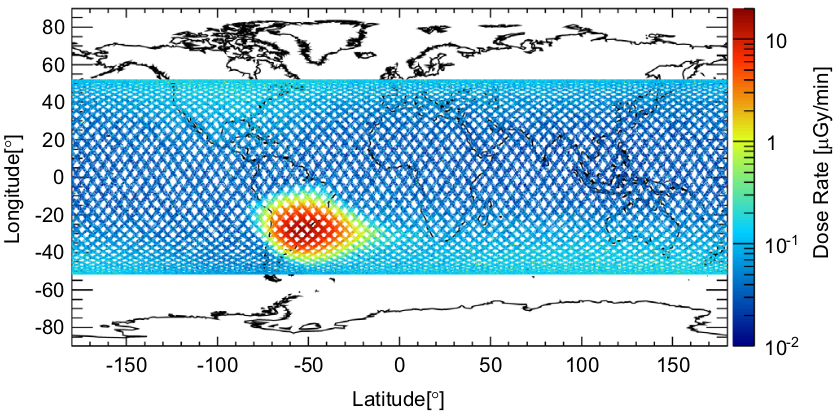
\includegraphics[width=0.48\textwidth]{./fig/plots/iss_map_2.png}
  }
  \caption{Ionizing radiation dose measured by the Timepix sensor onboard (a) VZLUSAT-1 ($\approx 500$\,km Sun-synchronous orbit), and (b) the \acl{ISS} ($\approx 350$\,km orbit).}
  \label{fig:intro_radiation_maps}
\end{figure}

%%}

We add to the list an embedded and lite-weight design of a Timepix payload for the first Czech CubeSat satellite, the VZLUSAT-1 \cite{urban2017vzlusat, daniel2019inorbit}.
The payload was dedicated to radiation mapping of Earth's \ac{LEO} \cite{baca2018timepix} and capturing images using the onboard X-Ray telescope \cite{baca2016miniaturized}.
The satellite has been operational for more than 3 years.
New radiation data are being processed on regular basis while being added to an open-source dataset\footnote{\url{https://github.com/vzlusat}} potentially useful for the community of future CubeSat designers.
Further research let to a design of a one-time sub-orbital rocket experiment \cite{daniel2017xray, urban2020rex}.
A dedicated payload with two Timepix sensors were designed and developed based upon the \acl{ROS} \cite{baca2018rospix}.
Embedded hardware with \ac{ROS} automatically managed recording of the measured data in real time.
This crossover of technologies later allowed to continue on the development of \ac{ROS}-based Timepix technologies for the use onboard \aclp{UAV}.

%%}

%%{ Localization and mapping of ionizing radiation sources by \acp{UAV}

\subsection{Localization and mapping of ionizing radiation sources by \acp{UAV}}

In radiation sensing, unmanned robotic vehicles offer several advantages over conventional handheld detectors or piloted aircraft.
These advantages can be exploited in a wide variety of applications.

Following the 2011 disaster at the \ac{FDNPP}, considerable amounts of radioactive material have been released into the plant area.
Several \acp{UGV} have been deployed directly inside the damaged reactor buildings of \ac{FDNPP} under remote control.
Various radiation detection methods have been tested inside the power plant, including a coded aperture scintillator \cite{ohno2011robotic}, a semiconductor digital dosimeter \cite{nagatani2013emergency}, a Compton event camera composed of two scintillators \cite{sato2019radiation}, and a time-of-flight gamma camera \cite{kinoshita2014development}.
Ground-based robots offer higher payload capacity and the ability to carry heavier sensory equipment than most aerial vehicles.
On the other hand, these robots tend to be relatively bulky, struggle to navigate the cluttered corridors and staircases inside the damaged buildings, and generally move slower than a multirotor aircraft.

\acp{UAV} have been utilized to map the spread of the radioactive material outside the power plant.
These range from large aircraft weighing more than \SI{90}{\kilogram} equipped with heavy scintillation detectors \cite{sanada2015aerial, towler2012radiation, jiang2016prototype}
to compact multi-rotors suitable for flying along a pre-defined trajectory close to the ground \cite{macfarlane2014lightweight, christie2017radiation, martin20163d}.
Outside of Japan, several projects have employed \acp{UAV} for radiation intensity mapping around uranium ore mines \cite{salek2018mapping, keatley2018source, martin2015use}.

In \cite{han2013lowcost}, multiple fixed-wing \acp{UAV} equipped with miniature scintillators are used for contour analysis of an irradiated area.
Trajectory planning and data processing are performed offline, contrary to our approach, which estimates the source's position in real-time during the flight.
In \cite{newaz2016uav}, the contour analysis is tackled using a single multirotor \ac{UAV}. The contour analysis uses a Gaussian mixture model to estimate multiple radiation sources' positions with overlapping intensity fields.
The projects mentioned above utilize unmanned vehicles to deliver a radiation sensor into a hazardous environment.
However, the approaches do not respond to measured data in real-time and thus do not exploit the mobility of \acp{UAV} to improve the measurement.

Active path-planning driven by the onboard measurements has been shown in \cite{towler2012radiation} for an outdoor environment and in \cite{mascarich2018radiation} for a GPS-denied indoor environment.
Both of these works rely on a scintillator sensor to estimate the radiation intensity in the \ac{UAV}'s current position.
As a result, the employed aerial platforms have to be large with a payload capacity exceeding \SI{2}{\kilogram}.
As in \cite{towler2012radiation}, the aerial platform is a \SI{90}{\kilogram} unmanned aerial helicopter, which significantly limits its deployment conditions due to personal safety and considerable minimum distance to obstacles in the environment.

The lack of lightweight radiation detectors with immediate readout capability severely limits the application potential of aerial dosimetry.
However, the Timepix pixel detectors are ideal for the use onboard micro \acp{UAV} thanks to their low weight, small size, and the absence of any active cooling mechanism.
We propose a \ac{UAV} system for outdoor and indoor environments while utilizing the know-how obtained with the embedded space applications' work.
The \ac{ROS} \acs{API} for Timepix \cite{baca2018rospix}, initially developed for a suborbital rocket experiment \cite{urban2020rex}, allows the technology transfer to the robotics field.
However, a new robotic methodology for motion planning and exploration needed to be developed to accommodate and utilize the proposed measurement system's specifics \cite{stibinger2020localization}.
Moreover, the Compton camera mechanism \cite{turecek2018compton}, is being utilized to provide the smallest real-time single-sensor Compton camera ever used on a \acp{UAV} \cite{baca2020gamma}.

%%{ Fig: example

\begin{figure}[!h]
  \centering
  \subfloat[Visualization of the localization] {
    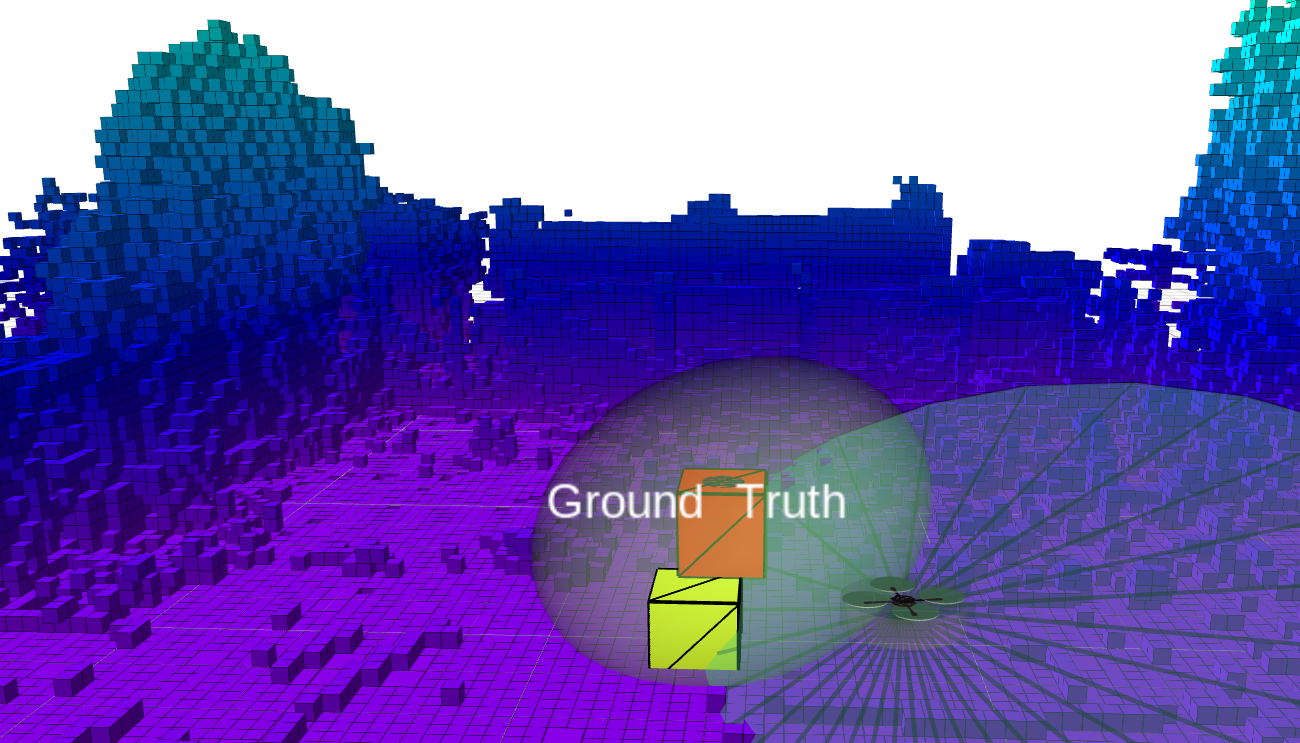
\includegraphics[width=0.415\textwidth]{./fig/plots/rviz_3d.png}
  }
  \subfloat[\ac{UAV} equipped with the Timepix3 sensor] {
    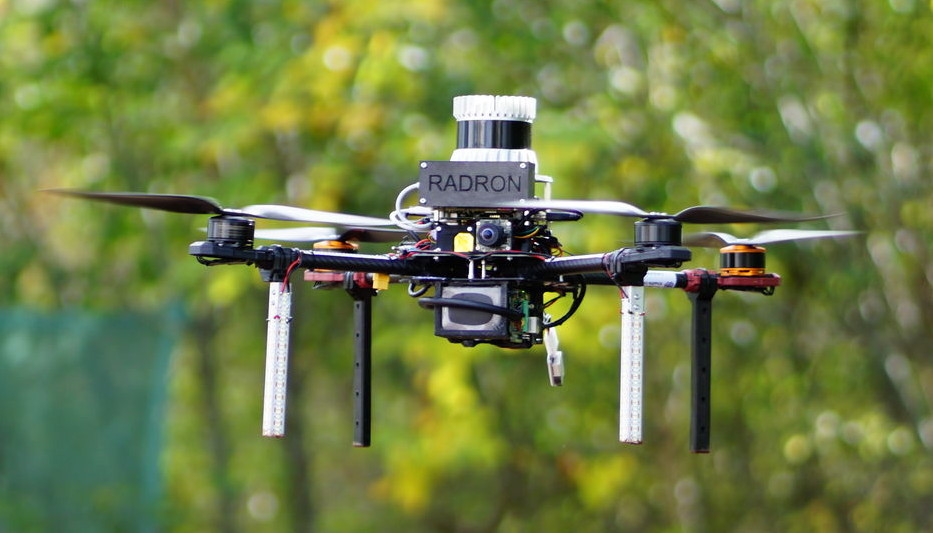
\includegraphics[width=0.415\textwidth]{./fig/photos/radron_uav.jpg}
  }
  \caption{Showcase from a radiation localization experiment with the MiniPIX Timepix3 Compton camera onboard a \ac{UAV}. The visualization shows the ground truth position of the radiation source (yellow) and the estimated position (red).}
  \label{fig:intro_uav_example}
\end{figure}

%%}

%%}

%%}

%%}

%% | ------------------------ Chapter 3 ----------------------- |

%%{ Research-focused UAV Platform

\chapter{Research-focused UAV Platform\label{chap:uav_platform}}

Our initial work on relatively-localized \ac{UAV} formations \cite{saska2013adhoc, chudoba2014localization} led us to create a custom platform for experimental evaluation.
This control system \cite{baca2016embedded} used an embedded \ac{MPC} controller executed in real time onboard in custom hardware.
This embedded system, in conjunction with the novel relative localization system \cite{krajnik2014practical}, allowed us to conduct our first multi-\ac{UAV} research that was backed up by real-world experiments \cite{saska2016formations, saska2017system, spurny2016complex, chudoba2016exploration}.

As the demands for the capabilities of the platform increased, we abandoned the embedded platform and adopted a modular approach of the \acl{ROS}.
The first core publication in this thesis, presented at the \acs{IEEE} IROS 2018 conference, proposes a model predictive tracking mechanism for fast generation of feasible control references for \acp{UAV}.
\fullciteinbox{baca2018model}{}
\noindent
Obtaining a feasible control reference that satisfies state constraints of the \ac{UAV} is an essential requirement for precise feedback control.
Moreover, the presented approach utilizes the \SI{8}{s} \ac{MPC} prediction horizon for a mutual \ac{UAV} collision avoidance, which is especially useful for the verification of new multi-\ac{UAV} methods.
The presented control technique was partially responsible for our success in the \ac{MBZIRC} 2018 robotic competition \cite{baca2019autonomous, loianno2018localization, spurny2019cooperative}.

The \emph{MPC Tracker} \cite{baca2018model}, is however just a small part of complex system for multirotor \ac{UAV} experimental evaluation and deployment.
With the second core publication in this thesis, we propose a modular control system for \ac{UAV} state estimation, trajectory tracking, feedback control, and flight management.
This open-source control system sets up novel paradigms, such as the multi-frame \ac{UAV} state estimation, the heading-based control pipeline devout of Euler and Tait-Bryan angles.
Testing new feedback controllers, reference generators, state estimators, and other parts of the control pipeline are possible thanks to the modular design and the extensive simulation environment.
The \emph{MRS UAV System} was submitted to the Journal of Intelligent \& Robotic Systems and is being available as open source\footnote{\url{https://github.com/ctu-mrs/mrs_uav_system}}.
\fullciteinbox{baca2020mrs}{}

\includepaperwithimage{baca2018model}
\includepaperwithimage{baca2020mrs}

%%}

%% | ------------------------ Chapter 4 ----------------------- |

%%{ Advances in remote sensing by UAVs

\chapter{Advances in remote sensing by UAVs\label{chap:sensing}}

The author of this thesis has contributed to various sub-fields of multi-\ac{UAV} research, inc. multi-\ac{UAV} swarming \cite{petracek2020bioinspired, saska2020formation, ahmad2020autonomous, dmytruk2020safe}, search and rescue \cite{roucek2019darpa, petrlik2020robust, kratky2020autonomous2}, planning and control \cite{penicka2017dubins, giernacki2019realtime, saikin2020wildfire, silano2020power, spurny2016complex}, and sensing \cite{stibinger2020localization, baca2018rospix, kratky2020autonomous2}.
However, most of the author's effort during his studies had been invested in the research scenarios proposed by the Khalifa University as the 2017 and 2020 \ac{MBZIRC} robotic challenges\footnote{\url{https://mbzirc.com}}.

The following core publication \cite{baca2019autonomous} in this thesis proposes a \ac{UAV} system for autonomous landing on a moving car.
This complete system was able to perform the fastest autonomous landing (\SI{25}{\second}) among all the teams competing in the challenge, using onboard sensors and computational power.
Onboard computer vision \cite{stepan2019vision} was employed to detect the car in wide \ac{FOV} monocular camera images and nonlinear state estimation based on \ac{UKF} was performed to predict the car's future motion.
The car was driving at the speed of \SI{15}{\kilo\meter\per\hour} in a designated area, following an 8-shaped path.
The system was evaluated extensively in simulations and various real-world conditions, and the final experiments were successfully performed in the constrained environment of the competition venue.
\fullciteinbox{baca2019autonomous}{}

The second challenge in \ac{MBZIRC} 2017 competition focused on the collaborative gathering of metal objects by a group of \acp{UAV}.
A team of 3 \acp{UAV} was tasked with gathering colored metal discs that were both stationary and moving (attached to ground mobile robots).
The challenge posed many subproblems, including onboard computer vision \cite{stepan2019vision}, sensor fusion, state estimation, feedback control, motion planning, robot coordination, and mechatronics.
All the subproblems needed to be addressed competently and efficiently to obtain any score within the competition.
The proposed system was tested extensively in simulations, and various outdoor conditions \cite{loianno2018localization}.
It performed consistently as the best solution to the challenge during the competition trials in Abu Dhabi.
The MRS team won the 1$^{\text{st}}$ place among prestigious university teams from all over the world.
The following core publication presents the system, its core features, and the experimental results.
\fullciteinbox{spurny2019cooperative}{}

The \ac{MBZIRC} 2020 challenge inspired the third core publication in this research stream (submitted to \emph{Robotics \& Autonomous Systems}, after the first revision).
The 2$^{\text{nd}}$ round of this competition focused again on \aclp{UAV} and extended the 1$^{\text{st}}$ 2017 challenge.
The article reports on the system for multi-robotic brick wall construction by a team of \acp{UAV}.
Although this task is similar to the 2017 object-gathering challenge, significant advances in \ac{UAV} control and state estimation were required to address the problem successfully.
Moreover, a novel multi-frame state estimation framework was proposed for seamless switching between globally-localized flight and an egomotion visual servoing \cite{baca2020mrs}.
This system allowed the use of true visual servoing to achieve pinpoint accuracy during the autonomous grasping maneuver.
The \acs{MRS} team won again the 1$^{\text{st}}$ place in the competition and showed again, by a significant margin, the best approach for solving the multi-robotic task.
\fullciteinbox{baca2020autonomous}{}

\includepaperwithimage{baca2019autonomous}
\includepaperwithimage{spurny2019cooperative}
\includepaperwithimage{baca2020autonomous}

%%}

%% | ------------------------ Chapter 5 ----------------------- |

%%{ Ionizing Radiation Detection and Localization by UAVs

\chapter{Ionizing Radiation Detection and Localization by UAVs\label{chap:radiation}}
\chaptermark{Ionizing Radiation Sources Localization}

The first core publication related to radiation mapping presents the results from the first year of the VZLUSAT-1 nanosatellite operation.
The satellite \cite{urban2017vzlusat} was launched in June, 2017 \cite{daniel2019inorbit}.
It carried, among other scientific instruments, a miniaturized X-ray telescope with the Timepix particle detector \cite{baca2016miniaturized}.
The author was responsible for the design, development, and commissioning of the satellite's payload and is responsible for the ongoing data acquisition and processing.
This research represents the author's first step into the community of particle imaging and radiation dosimetry.
Without these contributions and gained know-how, the following work on radiation localization and mapping by \acp{UAV} would probably have not been possible.
Furthermore, one of the tangents of this outer space research is the author's involvement in one of NASA's suborbital rocket flights \cite{miles2017introduction, wages2019flight, daniel2017xray}.
The thesis author designed a hardware readout interface and software, based on the \acl{ROS} \cite{baca2018rospix}, for two Timepix detectors onboard a sounding sub-orbital rocket \cite{urban2020rex}.
The following article presents the results of 1-year of orbital radiation measurements onboard the VZLUSAT-1 nanosatellite using the Timepix sensor.
\fullciteinbox{baca2018timepix}{}

The second core publication in this field provides an overview of potential utilization of the Timepix particle imaging detector in the field of \aclp{UAV}.
The article discusses the detector's critical properties and their relation to various methods of obtaining a directional measurement of a radiation source, such as pinhole apertures, X-ray optics, and collimators.
A method for real-time classification of the measured particle tracks is proposed.
The proposed classifier and \ac{ROS} drivers for the Timepix detector are provided as open-source.
Furthermore, it is concluded that the Compton camera principle shows promising properties, and a real-time Monte-Carlo simulation model for the Compton camera is presented.
\fullciteinbox{baca2019timepix}{}

The next core publication in this field focuses on distributed localization of ionizing radiation sources using multiple \acp{UAV} equipped with the Timepix sensor.
This work presents real-time radiation source localization and estimation methods for \acp{UAV} equipped with the Timepix sensors.
A path planning approach that exploits the asymmetrical intensity measurement response of the Timepix detector was proposed.
The approach uses multiple \acp{UAV} and their ability to vary the orientation of the sensor in space to estimate the direction to the radiation source.
Moreover, the work presents verification of real-world measurements onboard a \ac{UAV} against the proposed real-time Monte-Carlo ray-tracing simulation model of the Timepix sensor.
Realistic simulations in the Gazebo/ROS robotic simulator demonstrate the feasibility of the method.
\fullciteinbox{stibinger2020localization}{}

\includepaperwithimage{baca2018timepix}
\includepaperwithimage{baca2019timepix}
\includepaperwithimage{stibinger2020localization}

%%}

%% | ------------------------ Chapter 6 ----------------------- |

%%{ Results and Discussion

\chapter{Discussion and Results\label{chap:results}}
\chaptermark{Discussion and Results}

In this chapter, we summarize the contributions presented in the core articles.
Furthermore, we provide a discussion in context with the remainder of the author's work.
Finally, we suggest future work in the context of the three research streams.

%%{ Research-focused UAV System

\section{Research-focused UAV System}

The proposed \ac{UAV} system \cite{baca2020mrs, baca2018model} provides students and researchers the means to develop and test new methods in the field of feedback control, tracking, estimation, and planning.
The system is modular and allows anyone to add new modules, safely tested in simulations and even during a real-world flight.
Moreover, the system can be used without changes for testing of high-level localization methods, mapping, planning, and multi-robot coordination.

The first of our contributions is the \acl{MPC} tracker \cite{baca2018model}.
Even now, more than four years after it was first developed, we have not yet found a viable substitute for the tracking mechanism.
The \ac{MPC} tracker provides a mechanism for real-time generation of feasible and smooth feedforward control reference from any time-parametrized input trajectory.
The tracker's output satisfies \ac{UAV} constraints even when the input trajectory is not feasible.
Moreover, the integrated mutual collision avoidance mechanism allows the safe deployment of multiple \acl{UAV} in outdoor conditions.

The MRS \ac{UAV} system \cite{baca2020mrs} comes with two controller designs --- extended \emph{SE(3) geometric tracking} \cite{lee2010geometric} for agile and aggressive flight, and the novel \emph{MPC controller} for stable flight in case of potentially unreliable \ac{UAV} state estimate.
However, the system can be easily extended with new control approaches as needed, thanks to its modularity.
UAV controllers' survey provides a rich list of potentially useful control techniques \cite{nascimento2019position}.
For example, a novel adaptive backstepping controller \cite{zhang2019robust, labbadi2019robust} may provide better performance during aggressive maneuvers, thanks to the included rotor drag compensation.
The proposed extension to \emph{geometric tracking on SE(3)} \cite{lee2010geometric} can be further improved with remarks from \cite{lee2013nonlinear} to provide robust control to bounded uncertainties.
Furthermore, nonlinear \ac{MPC} controllers are becoming popular \cite{nascimento2019nmpc, pereira2019nonlinear, kamel2017robust}, thanks to their inherent ability to cope with complex constraints.
However, when dealing with theoretical work and experimental deployment in real-world conditions, we favor practicality over complexity.
We, therefore, utilize relatively simple controllers \cite{baca2020mrs}, with tractable inner mechanisms.

We summarize the novel properties of the proposed control system as
\begin{itemize}
  \item the previously-published \ac{MPC} tracker for control reference generation \cite{baca2018model},
  \item a novel bank-of-filters estimator design that overcomes challenges with diverse sensory equipment,
  \item a heading-oriented control design, devoid of ambiguous use of Euler/Tait-Bryan angles,
  \item a body/world disturbance estimation approach that does not rely on a specific state estimator design,
  \item a reliable MPC-based controller with the benefits of the nonlinear \emph{SO(3)} force feedback,
  \item a system that can be employed with a variety of onboard localization systems and sensors,
  \item the system can receive references in coordinate frames, which differ from the feedback loop reference frame.
\end{itemize}

The system has been used no only for research testing and evaluation but also for education and teaching.
We utilized the system for practical exercises during the 2019 and 2020 \acs{IEEE} \acs{RAS} Summer School on Multi-Robot Systems\footnote{\url{http://mrs.felk.cvut.cz/summer-school-2020}}.
Over a hundred students used the system while solving the tasks of multi-\ac{UAV} traveling salesman problem with neighborhoods (2019) and relatively-localized leader-follower flight with two \acp{UAV} (2020).

The future work on the MRS UAV system is currently foreseen as mostly implementation improvements, including the transition to \acs{ROS}2, and continuous improvement of the system's documentation.
However, some research topics remain.
The heading-based control approach should be generalized to allow the user to specify a vector in the \ac{UAV}'s body frame that represents the \ac{UAV} \emph{front}, other than the currently-used principle x-axis.
The azimuth of this vector should be considered as the heading.
This would allow precise tracking and control of the heading with respect to, e.g., an arbitrary optical axis of a camera mounted on the \ac{UAV}.
Without such a mechanism, the heading control relative to other than the \ac{UAV} body's x-axis can be achieved only approximately and with notable errors, especially during aggressive maneuvers.
However, this mechanism needs to be incorporated in both control and reference generation.
It must guarantee smooth control references and control actions even when the definition of the \ac{UAV}'s \emph{front} changes.

%%}

%%{ Advances in remote sensing by UAVs

\section{Advances in remote sensing by UAVs}

The \ac{UAV} tasks tackled within the core publications in this thesis were on the edge of field robotics in their time.
We successfully showed a multi-robotic system for autonomous object gathering \cite{spurny2019cooperative} and autonomous wall construction \cite{baca2020autonomous} by \acp{UAV}.
Both systems were put to the test during the \ac{MBZIRC} 2017 and \ac{MBZIRC} 2020 robotics competition, and both achieved first place among respected university teams from all over the world.
We also investigated the task of autonomous landing with a \ac{UAV} on top of a moving car \cite{baca2019autonomous} with the total second place in the competition and the fastest autonomous landing time among all the competing teams.
This robotics problem might be in the future a part of automatic remote sensing applications with \acp{UAV} being deployed and recovered by a car.
Each of the three problems brought us further in understanding the caveats of onboard state estimation, computer vision, control, and planning.
The important lesson we learned about robotics from our endeavors is the danger of overly focusing on one or a few specializations.
\ac{UAV} autonomy is a complex cybernetics field that encompasses many interconnected sub-fields.
We found that researchers often focus too narrowly on one of the sub-fields while ignoring the influence between other components of a whole autonomous system.
This can make the approaches narrow-minded and detached from reality and potentially not applicable to a real-world robotics system.

Although the particular problems solved in \cite{baca2019autonomous, spurny2019cooperative, baca2020autonomous} are probably not going to be pursued in the future by our team, the acquired know-how and knowledge are transferable to other applications.
We also pursue the \ac{DARPA} Subterranean competition on multi-robotic autonomous localization of objects and people in underground environments \cite{roucek2019darpa, kratky2020autonomous2, petrlik2020robust}.
Furthermore, our primary research on relatively-localized multi-\ac{UAV} swarms \cite{petracek2020bioinspired, saska2020formation, ahmad2020autonomous, dmytruk2020safe} benefits significantly from the systems and expertise we obtained in experimental field robotics.
Finally, the following section discusses the current contributions and our future work in the remote sensing sub-field of ionizing radiation sources.

%%}

%%{ Ionizing Radiation Detection and Localization by UAVs

\section{Ionizing Radiation Detection and Localization by UAVs}

We have come to the field of ionizing radiation detection from a different direction and using a different perspective than the rest of the \ac{UAV} community, specifically from the constrained environment of miniature space technologies \cite{baca2016miniaturized, baca2018timepix}.
Where the rest of the community often attempts to mount as large radiation detectors as possibly to a \ac{UAV} (to maximize measured counts-per-second), we strive towards minimizing both the sensor and the \ac{UAV} to deploy the \ac{UAV} in tightly constraint environments.
We can close the distance to the radiation source even in a cluttered environment and, therefore, obtain even more information, thanks to the inverse square law of radiation intensity over distance.
The concept of obtaining as much information as possible using large detectors is prominent throughout state of the art.
However, multiple factors should be considered when building an autonomous aerial system for radiation source localization.
We identified the following four factors:
\begin{itemize}
  \item detector size,
  \item aircraft size,
  \item environmental constraints,
  \item localization strategy.
\end{itemize}
As depicted in Figure~\ref{fig:radiation_cycle}, these four factors influence each other in a loop.
With a larger sensor comes a higher event count rate, which is understandably preferred by physicists.
However, large and heavy sensors require larger aircraft with higher payload capacity.
The aircraft size dictates its motion constraints through an environment; larger aircraft fly higher above the terrain and need increased safety distance from obstacles.
Those constraints determined the search strategy that, in turn, typically favors sensors with higher sensitivity; therefore, sensors with a larger mass.
The current state of the art does not break from this cycle in more than a couple of factors.
On the contrary, state of the art mostly utilizes \acp{UAV} just as a sensor carrier.
However, we conjecture that all four factors need to be adjusted simultaneously to show a breakthrough in the field.
In other words, the system needs to be developed while focusing on the specifics of sensors and the \acp{UAV} autonomy.

Making the sensor smaller will lower its weight as well as the raw count-per-second information yield.
However, miniature sensors can be mounted on an \ac{MAV} that can safely fly much closer to environmental obstacles.
Flying close to obstacles requires more intelligent onboard autonomy, sensing the obstacles and planning the \ac{UAV} motion with respect to the environment.
Proximity to obstacles opens new possibilities for search strategies, which can utilize the abilities of today autonomous systems and the potential to close the distance to the radiation source autonomously.
We aim to make such a breakthrough with know-how in both research fields.

%%{ endless circle diagram

\begin{figure}
  \begin{adjustbox}{max totalsize={1.0\textwidth}{0.90\textheight}, center}

    %%{ tikzset

    \tikzset{
      >=stealth',
      punkt/.style={
        rectangle,
        rounded corners,
        draw=black, very thick,
        text width=5.7em,
        minimum height=2em,
        text centered},
      just_text/.style={
        rectangle,
        text width=10.0em,
        minimum height=2em,
        text centered},
      small_punkt/.style={
        rectangle,
        rounded corners,
        draw=black, very thick,
        text width=4.0em,
        text centered},
      arrow/.style={
        ->,
        very thick,
        shorten <=2pt,
        shorten >=2pt,},
      arrow_gray/.style={
        ->,
        color=gray, very thick,
        shorten <=2pt,
        shorten >=2pt,},
      arrow_red/.style={
        ->,
        draw=red, very thick,
        shorten <=2pt,
        shorten >=2pt,}
      }

    %%}

    %%{ tikzfigure

    \begin{tikzpicture}[node distance=1cm, auto,]

      % outer circle nodes
      \node[punkt] (sensor) {Sensor size};

      \node[punkt, inner sep=5pt, below = of sensor, shift = {(-6.0, -0.75)}] (aircraft) {Aircraft\\size};

      \node[punkt, inner sep=5pt, below = of sensor, shift = {(0.0, -4.0)}] (constraints) {Environment constraints};

      \node[punkt, inner sep=5pt, below = of sensor, shift = {(6.0, -0.75)}] (strategy) {Localization strategy};

      % inner circle nodes
      \node[small_punkt, inner sep=5pt, below = of sensor, shift = {(0.0, 0.5)}] (sensor2) {\scriptsize Sensor size};

      \node[small_punkt, inner sep=5pt, right = of aircraft, shift = {(0.5, -0.0)}] (aircraft2) {\scriptsize Aircraft\\size};

      \node[small_punkt, inner sep=5pt, above = of constraints, shift = {(0.0, -0.5)}] (constraints2) {\scriptsize Environment\\constraints};

      \node[small_punkt, inner sep=5pt, left = of strategy, shift = {(-0.5, -0.0)}] (strategy2) {\scriptsize Localization\\strategy};

      % We make a dummy figure to make everything look nice.
      \path[->] ($(sensor.west)+(0, 0)$) edge [arrow,bend right=45] ($(aircraft.north)$);

      % \path[->] ($(sensor2.west)+(0, 0)$) edge [arrow, bend right=45, dashed] ($(aircraft.north)+(0.5, 0.0)$);

      \path[->] ($(aircraft.south)+(0, 0)$) edge [arrow,bend right=45] ($(constraints.west)$);

      \path[->] ($(constraints.east)+(0, 0)$) edge [arrow,bend right=45] ($(strategy.south)$);

      \path[->] ($(strategy.north)+(0, 0)$) edge [arrow,bend right=45] ($(sensor.east)$);

      % inner circle paths
      \path[->] ($(sensor2.west)+(0, 0)$) edge [arrow_red, bend right=45, dashed] ($(aircraft2.north)+(0.0, 0.0)$);

      \path[->] ($(aircraft2.south)+(0, 0)$) edge [arrow_red, bend right=45, dashed] ($(constraints2.west)+(0.0, 0.0)$);

      \path[->] ($(constraints2.east)+(0, 0)$) edge [arrow_red, bend right=45, dashed] ($(strategy2.south)+(0.0, 0.0)$);

      \path[->] ($(strategy2.north)+(0, 0)$) edge [arrow_red, bend right=45, dashed] ($(sensor2.east)+(0.0, 0.0)$);

      % % most outer arrows
      % \path[->] ($(sensor.north)+(0, 0)$) edge [arrow] ($(sensor.north)+(0.0, 0.5)$);
      % \path[->] ($(aircraft.west)+(0, 0)$) edge [arrow] ($(aircraft.west)+(-0.5, 0.0)$);
      % \path[->] ($(constraints.south)+(0, 0)$) edge [arrow] ($(constraints.south)+(0.0, -0.5)$);
      % \path[->] ($(strategy.east)+(0, 0)$) edge [arrow] ($(strategy.east)+(0.5, 0.0)$);

      % outer inner arrows
      \draw [->] ($(sensor.south)+(0, 0)$) -- ($(sensor2.north)$) node [midway, shift = {(0.0, 0.0em)}] {smaller};
      \draw [->] ($(aircraft.east)+(0, 0)$) -- ($(aircraft2.west)+(0.0, 0.0)$) node [midway, shift = {(0.0, 0.0em)}] {smaller};
      \draw [->] ($(constraints.north)+(0, 0)$) -- ($(constraints2.south)+(0.0, 0.0)$) node [midway, shift = {(0.0, 0.0em)}] {more complex};
      \draw [->] ($(strategy.west)+(0, 0)$) -- ($(strategy2.east)+(0.0, 0.0)$) node [midway, shift = {(0.0, 0.0em)}] {smarter};

      % \node[just_text, inner sep=5pt, below = of sensor, shift = {(0, -3.0)}] (text1) {\huge 2 kg};
      % \node[just_text, inner sep=5pt, below = of sensor, shift = {(0, -3.0)}] (text2) {\huge 10 kg};
      % \node[just_text, inner sep=5pt, below = of sensor, shift = {(0, -3.0)}] (text3) {\huge 100 m clearance};
      % \node[just_text, inner sep=5pt, below = of sensor, shift = {(0, -3.0)}] (text5) {\huge pre-planned scanning \& ex-post processing};
      % \node[just_text, inner sep=5pt, below = of sensor, shift = {(0, -3.0)}] (text6) {\huge 100 g};
      % \node[just_text, inner sep=5pt, below = of sensor, shift = {(0, -3.0)}] (text6) {\huge 1.5 kg};
      % \node[just_text, inner sep=5pt, below = of sensor, shift = {(0, -3.0)}] (text6) {\huge 5 m\\clerance};
      % \node[just_text, inner sep=5pt, below = of sensor, shift = {(0, -3.0)}] (text6) {\huge Onboard\\AI};

    \end{tikzpicture}

    %%}

  \end{adjustbox}

  \caption{The four interconnected factors of an autonomous aircraft system for localization of ionizing radiation sources. All four factors need to be adjusted simultaneously to introduce a breakthrough in the field (the smaller red cycle).}
  \label{fig:radiation_cycle}

\end{figure}

%%}

We have made contributions that allow us to employ the innovative Timepix sensors and Timepix3 event cameras onboard \acp{UAV}.
We proposed the Rospix\footnote{\url{https://github.com/rospix}} interface \cite{baca2018rospix} for the \acl{ROS} together with a particle classification pipeline \cite{baca2019timepix}.
The software and tools available for the Timepix family of detectors is dedicated solely for laboratory use and expect a human in the loop.
Any specific application outside of the intended use requires specific hardware and software to be developed in collaboration with the sensor interface manufacturer, as it was, e.g., for the VZLUSAT-1 nanosatellite \cite{baca2016embedded}.
The \ac{ROS} tools provided through Rospix allow full automation using standard tools within the robotics community.
Moreover, the particle classification pipeline is the first to be executable during the data acquisition and is available as open-source.
The classification pipeline was trained using diverse radiation data gathered by the VZLUSAT-1 nanosatellite mission \cite{baca2018timepix}.

Our first contributions related to the radiation dosimetry onboard \acp{UAV} consists of the review of radiation localization options for \acl{UAV}, the particle classification pipeline, and a real-time Monte Carlo ray-tracing model for a dual-sensor Compton camera \cite{baca2019timepix}.
Furthermore, we investigate the use of the bare Timepix sensor for multi-robotic localization of compact radiation sources \cite{stibinger2020localization} without a specialized mechanism to deduce a direction to the source.
We show the approach's potential using realistic robotic simulations and a real-time Monte Carlo ray-tracing model of gamma radiation.

The previously mentioned contributions were motivation and a precursor for the project proposal for the Technology Agency of the Czech Republic.
Such interdisciplinary tasks as the localization of ionizing radiation sources can be challenging to accomplish by an institution specializing in either field.
Therefore, the thesis author co-wrote a project proposal, together with \emph{Advacam, s.r.o.}, and the \emph{Czech Metrology Institute} would allow us to focus on the topic and dedicate more resources to the research.
Project no. FW01010317 (2020 -- 2022, 8$^{\text{th}}$ of 396 submitted for the call\footnote{\url{https://www.tacr.cz/soutez/program-trend/prvni-verejna-soutez-trend}}) called ``\textit{RADRON: Localization of ionizing radiation sources using small unmanned helicopters equipped with a Compton camera detector}'', co-written by the thesis author, focuses on utilizing the unique properties of the Timepix3 event cameras for real-time localization and tracking of compact radiation sources.
First project results, submitted to \emph{IEEE ICRA} \cite{baca2020gamma}, show the Timepix3 event camera used as a single-detector Compton camera onboard a \ac{UAV}.
The system was able to localize a relatively weak gamma source using only onboard sensors.
\fullciteinbox{baca2020gamma}{}
The future work in this research field is co-aligned with the project goals.
We focus on developing an \ac{MAV} equipped with a Compton camera based on the Timepix3 technology.
We aim at combining the Compton camera principle \cite{baca2020gamma} for localization of compact gamma sources, together with the count-based system \cite{stibinger2020localization} that can be utilized for ionizing charged particles.

%%}

%%}

%% | ------------------------ Chapter 7 ----------------------- |

%%{ Conclusion

\chapter{Conclusion}

This thesis addressed collaborative remote sensing by a group of \aclp{UAV}.
First, we focused on developing a \ac{UAV} control system for experimental evaluation of new methods in realistic real-world conditions.
The proposed system utilizes an \ac{MPC} tracking approach for generating feedforward control reference provides a modular control pipeline.
A novel feedback controller design combining an \ac{MPC} with geometric tracking controller on \emph{SO(3)} was proposed, together with a heading-based orientation system that is devout of the convention of Euler and Tait-Bryan angles.
The control system had been extensively tested throughout the years and provided the means for other research to be conducted.
One of the many uses of the system was during the 2017 and 2020 \ac{MBZIRC} robotics competition.
We tackled several problems on the edge of state of the art in field robotics at the time.
Our solutions to the problems of multi-\ac{UAV} object gathering and multi-\ac{UAV} brick wall construction showed the be the best in the world, and our solution to the autonomous landing on a moving car with a \ac{UAV} performed the fastest landing among the competitors.
This thesis's collection of core publications reports on complex cybernetics problems of feedback control, estimation, sensor fusion, computer vision, planning, and mechatronics sub-fields of aerial robotics.
Finally, we present contributions in the field of aerial localization of ionizing radiation sources.
We made the first steps into adopting the Timepix family of \ac{CMOS} hybrid semiconductor sensors to be used onboard a mobile robot.
We showed the sensors' properties, provide essential tools for their use onboard a robot, and suggested a methodology for their application.
First experiments were conducted with the Timepix and Timepix3 sensors onboard a \ac{UAV}.
Our latest results --- the first results of an ongoing project --- showed a successful use of the Timepix3 event camera in the form of Compton camera onboard a \ac{UAV} for localization of a compact gamma radiation source.

%%}

%% | ----------------------- References ----------------------- |

%%{ References

\appendix
\renewcommand\chaptername{Appendix}

\chapter{References}

References to the author's work are listed first, followed by other references cited within this work.
The references contain the author's contribution and the number of citations based on Web~of~Science~(WoS), Scopus, and Google Scholar~(GS).
The author has reached h-index 7.
The citation counts were gathered on January 1$^{\text{st}}$, 2021.

%%{ Core publications

\section{Thesis core publications}

\subsection*{Core articles in peer-reviewed journals}
\printbibliography[keyword={mine},keyword={phd_related},keyword={journal},keyword={core},notkeyword={submitted},heading=none,title={}]

\subsection*{Core conference articles}
\printbibliography[keyword={mine},keyword={phd_related},keyword={conference},keyword={core},notkeyword={submitted},heading=none,title={}]

\subsection*{Core articles --- submitted}
\printbibliography[keyword={mine},keyword={phd_related},keyword={submitted},keyword={core},heading=none,title={}]

%%}

%%{ Related publications

\section{Thesis-related author's publications}

\subsection*{Thesis-related articles in peer-reviewed journals}
\printbibliography[keyword={mine},keyword={phd_related},keyword={journal},notkeyword={core},notkeyword={submitted},heading=none,title={}]

% \subsection*{Thesis-related articles in peer-reviewed journals only with CiteScore~(CS)}
% \printbibliography[keyword={mine},keyword={phd_related},keyword={journal},keyword={cs},heading=none,title={}]

\subsection*{Thesis-related conference articles}
\printbibliography[keyword={mine},keyword={phd_related},keyword={conference},notkeyword={core},notkeyword={submitted},heading=none,title={}]

\subsection*{Thesis-related publications --- submitted}
\printbibliography[keyword={mine},keyword={phd_related},keyword={submitted},notkeyword={core},heading=none,title={}]

%%}

%%{ Partially-related publications

\section{Partially-related author's publications}

\subsection*{Partially-related articles in peer-reviewed journals}
\printbibliography[keyword={mine},keyword={phd_unrelated},keyword={journal},notkeyword={core},notkeyword={submitted},heading=none,title={}]

\subsection*{Partially-related conference articles}
\printbibliography[keyword={mine},keyword={phd_unrelated},keyword={conference},notkeyword={core},notkeyword={submitted},heading=none,title={}]

\subsection*{Partially-related publications --- submitted}
\printbibliography[keyword={mine},keyword={phd_unrelated},keyword={submitted},heading=none,title={}]

%%}

%%{ unrelated publications

\section{Unrelated author's publications}

\printbibliography[keyword={mine},notkeyword={phd_unrelated},notkeyword={phd_related},heading=none,title={}]

%%}

%%{ Cited references

\section{Cited references}
\printbibliography[notkeyword=mine,heading=none,title={}]

%%}

%%}

%% | ------------------------ Apendices ----------------------- |

%%{ Apendices

\appendix
\renewcommand\chaptername{Citations of author's publications}

\chapter{Citations of author's publications}

Citations of the author's work were extracted from the Web~of~Science.
First- and second-order self-citations are excluded.
The data were gathered on January 1$^{\text{st}}$, 2021.
\\

\DeclareCiteCommand{\fullcite}
{\usebibmacro{prenote}}
{\clearfield{addendum}%
  \usedriver
  {\defcounter{minnames}{6}%
  \defcounter{maxnames}{6}}
{\thefield{entrytype}}}
{\multicitedelim}
{\usebibmacro{postnote}}

\fullciteinbox{saska2017system}{}
\begin{refsection}[citations/no_autocit/saska2017system.bib]
  \nocite{*}
  \printbibliography[heading=none,title={},env=favoritebib]
\end{refsection}

% \fullciteinbox{faigl2017onsolution}{}
% \begin{refsection}[citations/no_autocit/faigl2017onsolution.bib]
%   \nocite{*}
%   \printbibliography[heading=none,title={},env=favoritebib]
% \end{refsection}

% \fullciteinbox{saska2016formations}{}
% \begin{refsection}[citations/no_autocit/saska2016formations.bib]
%   \nocite{*}
%   \printbibliography[heading=none,title={},env=favoritebib]
% \end{refsection}

\fullciteinbox{loianno2018localization}{}
\begin{refsection}[citations/no_autocit/loianno2018localization.bib]
  \nocite{*}
  \printbibliography[heading=none,title={},env=favoritebib]
\end{refsection}

\fullciteinbox{baca2016miniaturized}{}
\begin{refsection}[citations/no_autocit/baca2016miniaturized.bib]
  \nocite{*}
  \printbibliography[heading=none,title={},env=favoritebib]
\end{refsection}

\fullciteinbox{spurny2019cooperative}{}
\begin{refsection}[citations/no_autocit/spurny2019cooperative.bib]
  \nocite{*}
  \printbibliography[heading=none,title={},env=favoritebib]
\end{refsection}

\fullciteinbox{daniel2016terrestrial}{}
\begin{refsection}[citations/no_autocit/daniel2016terrestrial.bib]
  \nocite{*}
  \printbibliography[heading=none,title={},env=favoritebib]
\end{refsection}

\fullciteinbox{baca2018model}{}
\begin{refsection}[citations/no_autocit/baca2018model.bib]
  \nocite{*}
  \printbibliography[heading=none,title={},env=favoritebib]
\end{refsection}

\fullciteinbox{baca2017autonomous}{}
\begin{refsection}[citations/no_autocit/baca2017autonomous.bib]
  \nocite{*}
  \printbibliography[heading=none,title={},env=favoritebib]
\end{refsection}

\fullciteinbox{daniel2017xray}{}
\begin{refsection}[citations/no_autocit/daniel2017xray.bib]
  \nocite{*}
  \printbibliography[heading=none,title={},env=favoritebib]
\end{refsection}

\fullciteinbox{urban2017vzlusat}{}
\begin{refsection}[citations/no_autocit/urban2017vzlusat.bib]
  \nocite{*}
  \printbibliography[heading=none,title={},env=favoritebib]
\end{refsection}

\fullciteinbox{baca2016embedded}{}
\begin{refsection}[citations/no_autocit/baca2016embedded.bib]
  \nocite{*}
  \printbibliography[heading=none,title={},env=favoritebib]
\end{refsection}

\fullciteinbox{baca2019autonomous}{}
\begin{refsection}[citations/no_autocit/baca2019autonomous.bib]
  \nocite{*}
  \printbibliography[heading=none,title={},env=favoritebib]
\end{refsection}

\fullciteinbox{saska2017documentation}{}
\begin{refsection}[citations/no_autocit/saska2017documentation.bib]
\nocite{*}
\printbibliography[heading=none,title={},env=favoritebib]
\end{refsection}

\fullciteinbox{giernacki2019realtime}{}
\begin{refsection}[citations/no_autocit/giernacki2019realtime.bib]
  \nocite{*}
  \printbibliography[heading=none,title={},env=favoritebib]
\end{refsection}

\fullciteinbox{chudoba2014localization}{}
\begin{refsection}[citations/no_autocit/chudoba2014localization.bib]
  \nocite{*}
  \printbibliography[heading=none,title={},env=favoritebib]
\end{refsection}

\fullciteinbox{saikin2020wildfire}{}
\begin{refsection}[citations/no_autocit/saikin2020wildfire.bib]
  \nocite{*}
  \printbibliography[heading=none,title={},env=favoritebib]
\end{refsection}

\fullciteinbox{daniel2019inorbit}{}
\begin{refsection}[citations/no_autocit/daniel2019inorbit.bib]
  \nocite{*}
  \printbibliography[heading=none,title={},env=favoritebib]
\end{refsection}

\fullciteinbox{baca2018timepix}{}
\begin{refsection}[citations/no_autocit/baca2018timepix.bib]
  \nocite{*}
  \printbibliography[heading=none,title={},env=favoritebib]
\end{refsection}

\fullciteinbox{baca2018rospix}{}
\begin{refsection}[citations/no_autocit/baca2018rospix.bib]
  \nocite{*}
  \printbibliography[heading=none,title={},env=favoritebib]
\end{refsection}

\fullciteinbox{spurny2016complex}{}
\begin{refsection}[citations/no_autocit/spurny2016complex.bib]
  \nocite{*}
  \printbibliography[heading=none,title={},env=favoritebib]
\end{refsection}

\fullciteinbox{chudoba2016exploration}{}
\begin{refsection}[citations/no_autocit/chudoba2016exploration.bib]
  \nocite{*}
  \printbibliography[heading=none,title={},env=favoritebib]
\end{refsection}

\fullciteinbox{petrlik2020robust}{}
\begin{refsection}[citations/no_autocit/petrlik2020robust.bib]
  \nocite{*}
  \printbibliography[heading=none,title={},env=favoritebib]
\end{refsection}

%%}

\end{document}
